% !TEX root = saveliev_physics_general_course_1.tex
%!TEX TS-program = pdflatex
%!TEX encoding = UTF-8 Unicode


\chapter{STATISTICAL PHYSICS}\label{chap:11}

\section{Information from the Theory of Probability}\label{sec:11_1}

Assume that we have a macroscopic system, \ie, a system formed by an enormous number of microparticles (molecules, atoms, ions, electrons), in a given state. Assume further that a quantity $x$ characteristic of the system can have the discrete values
\begin{equation*}
	x_1, x_2, \ldots, x_i, \ldots, x_k, \ldots, x_s.
\end{equation*}

Let us make a very great number $N$ of measurements of the quantity $x$, bringing the system before each measurement to the same initial state. Instead of performing repeated measurements of the same system, we can take $N$ identical systems in the same state and measure the quantity $x$ once in all these systems. Such a set of identical systems in an identical state is called a \textbf{statistical ensemble}.

Assume that $N_1$ measurements gave the result $x_1$, $N_2$ measurements the result $x_2$,\ldots, $N_i$ measurements the result $x_i$ and so on ($\sum_i N_i=N$ is the number of systems in the ensemble). The quantity $N_i/N$ is defined as the \textbf{relative frequency} of appearance of the result $x_i$, while the limit of this quantity obtained when $N$ tends to infinity, \ie,
\begin{equation}\label{eq:11_1}
	P_i = \lim_{N\to\infty} \frac{N_i}{N}
\end{equation}

\noindent
is called the \textbf{probability of appearance of the result} $x_i$. In the following, in order to simplify the equations, we shall write the expression for the probability in the form $N_i/N$, bearing in mind that the transition to the limit is performed at $N\to\infty$.

Since $\sum_i N_i=N$, we have
\begin{equation}\label{eq:11_2}
	\sum_i P_i = \sum_i \frac{N_i}{N} = 1
\end{equation}

\noindent
\ie, the sum of the probabilities of all possible results of measurement equals unity.

The probability of obtaining the result $x_i$ or $x_k$ is
\begin{equation*}
	P_{i\text{ or }k} = \frac{N_i + N_k}{N} = \frac{N_i}{N} + \frac{N_k}{N} = P_i + P_k.
\end{equation*}

\noindent
We have thus arrived at the \textbf{theorem of summation of probabilities}. It states that
\begin{equation}\label{eq:11_3}
	P_{i\text{ or }k} = P_i + P_k.
\end{equation}

Assume that a system is characterized by the values of two quantities $x$ and $y$. Both quantities can take on discrete values whose probabilities of appearance are
\begin{equation*}
	P(x_i) = \frac{N(x_i)}{N},\quad P(y_k) = \frac{N(y_k)}{N}.
\end{equation*}

\noindent
Let us find the probability $P(x_i,y_k)$ of the fact that a certain measurement will give the result $x_i$ for $x$ and $y_k$ for $y$. The result $x_i$ is obtained in a number of measurements equal to $N(x_i)=P(x_i)N$. If the value of the quantity $y$ does not depend on that of $x$, then the result $y_k$ will be obtained simultaneously with $x_i$ in a number of cases equal to
\begin{equation*}
	N(x_i,y_k) = N(x_i) P(y_k) = [P(x_i) N] P(y_k)
\end{equation*}

\noindent
[$N(x_i)$ plays the part of $N$ for $y$]. The required probability is
\begin{equation*}
	P(x_i,y_k) = \frac{N(x_i,y_k)}{N} = P(x_i) P(y_k).
\end{equation*}

\noindent
Now we have arrived at the \textbf{theorem of multiplication of probabilities} according to which \textit{the probability of the simultaneous occurrence of statistically independent events equals the product of the probabilities of each of them occurring separately}:
\begin{equation}\label{eq:11_4}
	P(x_i,y_k) = P(x_i) P(y_k).
\end{equation}

Knowing the probability of the appearance of different measurement results, we can find the mean value of all the results. According to the definition of the mean value
\begin{equation}\label{eq:11_5}
	\average{x} = \frac{1}{N}\sum_i N_i x_i = \sum_i P_i x_i.
\end{equation}

Let us extend the results obtained to the case when the quantity $x$ characterizing a system can take on a continuous series of values from zero to infinity. In this case, the quantity $x$ is said to have a continuous spectrum of values (in the previous case the spectrum of values was discrete).

Let us take a very small quantity $a$ (say, $a=\num{e-6}$) and find the number of measurements $\Delta N_0$ which give $0<x<a$, the number $\Delta N_1$ which give $a<x<2a$, \ldots, the number $\Delta N_x$ for which the result of the measurements is within the interval from $x$ to $x+a$, and so on. The probability of the fact that the result of the measurements will be within the interval from zero to a is $\Delta P_0=\Delta N_0/N$, within the interval from $a$ to $2a$ is $\Delta P_1=\Delta N_1/N$, \ldots, within the interval from $x$ to $x+a$ is $\Delta P_x=\Delta N_x/N$. Let us draw an $x$-axis and lay off strips of width $a$ and of height $\Delta P_x/a$ upward from it (\fig{11_1}a). We obtain a \textbf{bar graph} or \textbf{histogram}. The area of the bar whose left-hand edge has the coordinate $x$ is $\Delta P_x$ and the area of the entire histogram is unity [see \eqn{11_2}].

\begin{figure}[t]
	\begin{center}
		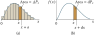
\includegraphics[scale=1.0]{figures/ch_11/fig_11_1.pdf}
		\caption[]{}
		\label{fig:11_1}
	\end{center}
	\vspace{-0.8cm}
\end{figure}

A histogram characterizes graphically the probability of obtaining results of measurements confined within different intervals of width $a$. The smaller the width of the interval $a$, the more detailed will the distribution of the probabilities of obtaining definite values of $x$ be characterized. In the limit when $a\to 0$, the stepped line confining the histogram transforms into a smooth curve (\fig{11_1}b). The function $f(x)$ defining this curve analytically is called a \textbf{probability distribution function}.

In accordance with the procedure followed in plotting the distribution curve, the area of the bar of width $\deriv{x}$ (see \fig{11_1}b) equals the probability of the fact that the result of a measurement will be within the range from $x$ to $x+\deriv{x}$. Denoting this probability by $\deriv{P_x}$ we can write that
\begin{equation}\label{eq:11_6}
	\deriv{P_x} = f(x)\,\deriv{x}.
\end{equation}

\noindent
The subscript ``x'' used with $\deriv{P}$ indicates that we have in mind the probability for the interval whose left-hand edge is at the point with the coordinate $x$. The area confined by a distribution curve, like that of a histogram, equals unity. This signifies that
\begin{equation}\label{eq:11_7}
	\int f(x)\,\deriv{x} = \int \deriv{P_x} = 1.
\end{equation}

\noindent
Integration is performed over the entire interval of possible values of the quantity $x$. Equation~\eqref{eq:11_7} is an analogue of \eqn{11_2}.

Knowing the distribution function $f(x)$, we can find the mean value of the results of measuring the quantity $x$. In $\deriv{N_x}=N\,\deriv{P_x}$ cases, a result equal to $x$ is obtained. The sum of such results is determined by the expression $x\,\deriv{N_x}=xN\,\deriv{P_x}$. The sum of all the possible results is $\int x\,\deriv{N_x}=\int xN\,\deriv{P_x}$. Dividing this sum by the number of measurements $N$, we get the mean value of the quanity $x$:
\begin{equation}\label{eq:11_8}
	\average{x} = \int x\,\deriv{P_x}.
\end{equation}

\noindent
This equation is an analogue of \eqn{11_5}.

Using \eqn{11_6} for $\deriv{P_x}$ in \eqn{11_8}, we obtain
\begin{equation}\label{eq:11_9}
	\average{x} = \int x f(x)\,\deriv{x}.
\end{equation}

Similar reasoning shows that the mean value of a function $\varphi(x)$ can be calculated by the equation
\begin{equation}\label{eq:11_10}
	\average{\varphi(x)} = \int \varphi(x) f(x)\,\deriv{x}.
\end{equation}

\noindent
For example,
\begin{equation}\label{eq:11_11}
	\average{x^2} = \int x^2 f(x)\,\deriv{x}.
\end{equation}

\section{Nature of the Thermal Motion of Molecules}\label{sec:11_2}

If a gas is in equilibrium, its molecules move absolutely without order, chaotically. All the directions of motion are equally probable, and none of them can be given preference over others. The velocities of the molecules may have the most diverse values. Upon each collision with other molecules, the magnitude of the velocity or speed of a given molecule should, generally speaking, change. It may grow or diminish with equal probability.

The velocities of molecules change by chance upon collisions. A molecule in a series of consecutive collisions may receive energy from its collision partners, and as a result its energy will considerably exceed the mean value $\average{\varepsilon}$. Even if we imagine the absolutely fantastic case, however, in which all the molecules of a gas give up their energy to a single molecule and stop moving, the energy of this molecule, and consequently its velocity too, will still be finite. Thus, the velocity of molecules of a gas cannot have values beginning with a certain $\ab{v}{max}$ and ending with infinity. Taking into consideration that processes which would lead to the concentration of a considerable portion of the total energy of all the molecules on one molecule have a low probability, we can say that very high velocities in comparison with the mean value of the velocity can be realized extremely rarely. In exactly the same way, it is virtually impossible for the velocity of a molecule to vanish completely as a result of collisions. Hence, very low and very high velocities in comparison with the mean value have a low probability. The probability of the given value of $v$ tends to zero both when $v$ tends to zero and when it tends to infinity. It thus follows that the velocities of molecules are mainly grouped near a certain most probable value.

\begin{figure}[t]
	\begin{center}
		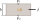
\includegraphics[scale=0.95]{figures/ch_11/fig_11_2.pdf}
		\caption[]{}
		\label{fig:11_2}
	\end{center}
	\vspace{-0.8cm}
\end{figure}

The chaotic nature of motion of molecules can be illustrated with the aid of the following procedure. Let us surround point $0$ with a sphere of arbitrary radius $r$ (\fig{11_2}). Any point A on this sphere determines the direction from $0$ to A. Consequently, the direction in which the molecules of a gas move at a certain moment can be set by points on the sphere. The equal probability of all the directions results in the fact that the points showing the directions of motion of the molecules will be distributed over the sphere with a constant density. The latter equals the number $N$ of molecules being considered divided by the surface area of the sphere $4\pi r^2$. Collisions lead to changes in the directions of motion of the molecules. As a result, the positions of the $N$ points on the sphere continuously change. Owing to the chaotic nature of the motion of the molecules, however, the density of the points at any spot on the sphere remains constant all the time.

The number of possible directions in space is infinitely great. But at each moment a finite number of directions is realized, equal to the number of molecules being considered. Therefore, putting the question of the number of molecules having a given (depicted by the point on the sphere) direction of motion is deprived of all meaning. Indeed, since the number of possible directions is infinitely great, whereas the number of molecules is finite, the probability of at least one molecule flying in a strictly definite direction equals zero. A question we are able to answer is what number of molecules move in directions close to the given one (determined by point A on the sphere). All the points of the surface elements $\Delta S$ of the sphere taken in the vicinity of point A (see \fig{11_2}) correspond to these directions. Since the points depicting the directions of motion of the molecules are distributed uniformly over the sphere, then the number of points within the area $\Delta S$ will be
\begin{equation}\label{eq:11_12}
	\Delta \ab{N}{A} = N\frac{\Delta S}{4\pi r^2}.
\end{equation}

\noindent
The subscript A indicates that we have in view the molecules whose directions of motion are close to that determined by point A.

The ratio $\Delta S/r$ is the solid angle $\Delta\Omega$ subtended by the area $\Delta S$.  Therefore, \eqn{11_12} can be written as follows:
\begin{equation}\label{eq:11_13}
	\Delta \ab{N}{A} = N\frac{\Delta\Omega}{4\pi}.
\end{equation}

\noindent
Here $\Delta\Omega$ is the solid angle containing the directions of motion of the molecules being considered. We remind our reader that $4\pi$ is a complete solid angle (corresponding to the entire surface of the sphere).

The direction of $0$A can be given with the aid of the polar angle $\theta$ and the azimuth $\varphi$ (\fig{11_3}). Hence, the directions of motion of the molecules of a gas can be characterized by giving for each molecule the values of the angles $\theta$ and $\varphi$ measured from a fixed direction $0$Z (we can take the direction of a normal to the surface of the vessel confining a gas as such a direction) and the plane P$_0$ drawn through it.

\begin{figure}[t]
	\begin{minipage}[t]{0.5\linewidth}
		\begin{center}
			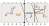
\includegraphics[scale=1.0]{figures/ch_11/fig_11_3.pdf}
			\caption[]{}
			\label{fig:11_3}
		\end{center}
	\end{minipage}
	\hspace{-0.05cm}
	\begin{minipage}[t]{0.5\linewidth}
		\begin{center}
			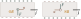
\includegraphics[scale=1.0]{figures/ch_11/fig_11_4.pdf}
			\caption[]{}
			\label{fig:11_4}
		\end{center}
	\end{minipage}
	\vspace{-0.4cm}
\end{figure}

Let us surround the origin of coordinates $0$ with a sphere of radius $r$ and find the element $\deriv{S}$ of the sphere corresponding to the increments $\deriv{\theta}$ and $\deriv{\varphi}$ of the angles $\theta$ and $\varphi$ (\fig{11_4}). The element being considered is a rectangle with the sides $r\,\deriv{\theta}$ and $r\sin\theta\,\deriv{\varphi}$. Thus,
\begin{equation}\label{eq:11_14}
	\deriv{S} = r^2 \sin\theta\,\deriv{\theta}\,\deriv{\varphi}.
\end{equation}

\noindent
The expression obtained gives an element of the surface $r=\text{constant}$ in a spherical system of coordinates.

Dividing \eqn{11_14} by $r^2$, we shall find the element of the solid angle corresponding to the angle intervals from $\theta$ to $\theta+\deriv{\theta}$ and from $\varphi$ to $\varphi+\deriv{\varphi}$:
\begin{equation}\label{eq:11_15}
	\deriv{\Omega_{\theta,\varphi}} = \sin\theta\, \deriv{\theta} \,\deriv{\varphi}.
\end{equation}

Two spheres of radii $r$ and $r+\deriv{r}$, two cones with the apex angles $\theta$ and $\theta+\deriv{\theta}$, and two planes forming the angles $\varphi$ and $\varphi+\deriv{\varphi}$ with P$_0$ separate in space a rectangular parallelepiped with the sides $r\,\deriv{\theta}$, $r\sin\theta\,\deriv{\varphi}$ and $\deriv{r}$ (see \fig{11_4}). The volume of this parallelepiped
\begin{equation}\label{eq:11_16}
	\deriv{V} = r^2\sin\theta\, \deriv{r}\, \deriv{\theta} \,\deriv{\varphi}
\end{equation}

\noindent
is an element of volume in a spherical system of coordinates (the volume corresponding to an increase in the coordinates $r$, $\theta$, and $\varphi$ by $\deriv{r}$, $\deriv{\theta}$ and $\deriv{\varphi}$).

Passing over from deltas to differentials in \eqn{11_13} and introducing \eqn{11_15} for $\deriv{\Omega}$, we arrive at the expression
\begin{equation}\label{eq:11_17}
	\deriv{N_{\theta,\varphi}} = N\frac{\deriv{\Omega_{\theta,\varphi}}}{4\pi} = N\frac{\sin\theta\,\deriv{\theta}\,\deriv{\varphi}}{4\pi}.
\end{equation}

\noindent
The subscripts $\theta$ and $\varphi$ of $\deriv{N}$ indicate that we have in view the molecules whose directions of motion correspond to the angle intervals from $\theta$ to $\theta+\deriv{\theta}$ and from $\varphi$ to $\varphi+\deriv{\varphi}$.

\section{Number of Collisions of Molecules with a Wall}\label{sec:11_3}

Let us consider a gas in equilibrium confined in a vessel. We shall take an element $\Delta S$ of the surface of the vessel and count the number of collisions of molecules with this element during the time $\Delta t$.

\begin{figure}[t]
	\begin{center}
		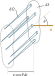
\includegraphics[scale=1.0]{figures/ch_11/fig_11_5.pdf}
		\caption[]{}
		\label{fig:11_5}
	\end{center}
	\vspace{-0.8cm}
\end{figure}

Let us separate from the $N$ molecules in the vessel those $\deriv{N_v}$ molecules whose velocities have magnitudes ranging from $v$ to $v+\deriv{v}$. Of these molecules, the number of molecules whose directions of motion are confined within the solid angle $\deriv{\Omega}$ equals
\begin{equation}\label{eq:11_18}
	\deriv{N_{v,\theta,\varphi}} = \deriv{N_v} \frac{\deriv{\Omega_{\theta,\varphi}}}{4\pi}
\end{equation}

\noindent
[see \eqn{11_17}]. Of the molecules separated in this way, the ones confined in an oblique cylinder with the base $\Delta S$ and the altitude $(v\cos\theta)\Delta t$ (\fig{11_15}) will fly during the time $\Delta t$ up to the area $\Delta S$ and collide with it\footnote{The objection could seem possible that part of these molecules would collide with other molecules on their way to the wall, as a result of which they will change their direction and will not reach the area $\Delta S$. These collisions, however, will not violate the chaotic nature of motion of the molecules: the transition of a certain number of molecules from the group moving toward the wall to groups moving in other directions is attended by the simultaneous transition of the number of molecules from the other groups to the one moving toward the wall. Consequently, in calculating the number of molecules reaching the wall, the collisions of the molecules with one another may be disregarded.}. The number of these molecules is
\begin{equation}\label{eq:11_19}
	\deriv{\nu_{v,\theta,\varphi}} = \deriv{N_v} \frac{\deriv{\Omega_{\theta,\varphi}}}{4\pi}\frac{\Delta S (v\cos\theta)\Delta t}{V}
\end{equation}

\noindent
($V$ is the volume of the vessel).

To obtain the total number of collisions of the molecules with the area $\Delta S$, we must summate \eqn{11_19} over the solid angle $2\pi$ (corresponding to changes in $\theta$ from $0$ to $\pi/2$ and changes in $\varphi$ from $0$ to $2\pi$) and over the velocities ranging from $0$ to $\ab{v}{max}$, where $\ab{v}{max}$ is the maximum velocity the molecules can have in the given conditions (see the preceding section).

We shall begin with summation over the directions. For this purpose, we shall write $\deriv{\Omega}$ in the form $\sin\theta\,\deriv{\theta}\,\deriv{\varphi}$ [see \eqn{11_15}] and integrate \eqn{11_19} with respect to $\theta$ within the limits from $0$ to $\pi/2$ and with respect to $\varphi$ within the limits from $0$ to $2\pi$:
\begin{equation*}
	\deriv{\nu_v} = \frac{\deriv{N_v} v \Delta S \Delta t}{4\pi V} \int_{0}^{\pi/2} \cos\theta\sin\theta\,\deriv{\theta} \int_{0}^{2\pi} \deriv{\varphi}.
\end{equation*}

\noindent
Integration with respect to $\deriv{\varphi}$ gives $2\pi$, and the integral with respect to $\deriv{\theta}$ equals $1/2$. Hence,
\begin{equation}\label{eq:11_20}
	\deriv{\nu_{v}} = \frac{\deriv{N_v} v \Delta S \Delta t}{4V}.
\end{equation}

\noindent
This expression gives the number of times the molecules flying in the directions confined within the solid angle $2\pi$ and having velocities from $v$ to $v+\deriv{v}$ collide with the area $\Delta S$ during the time $\Delta t$.

Summation over the velocities gives the total number of collisions of the mole-cules with the area $\Delta S$ during the time $\Delta t$:
\begin{equation}\label{eq:11_21}
	\nu_{\Delta S,\Delta t} = \frac{\Delta S \Delta t}{4V} \int_{0}^{\ab{v}{max}} v\,\deriv{N_v}.
\end{equation}

\noindent
The expression
\begin{equation*}
	\frac{1}{N}\int_{0}^{\ab{v}{max}} v\,\deriv{N_v}
\end{equation*}

\noindent
is the mean value of the speed $v$. Substituting the product $N\average{v}$ for the integral in \eqn{11_21}, we find that
\begin{equation}\label{eq:11_22}
	\nu_{\Delta S,\Delta t} = \frac{\Delta S \Delta t}{4V} N\average{v} = \frac{1}{4}n \average{v}\Delta S \Delta t.
\end{equation}

\noindent
Here $n=N/V$ is the number of molecules of a gas in unit volume.

Finally, dividing \eqn{11_22} by $\Delta S$ and $\Delta t$, we shall find the number of collisions of the gas molecules with a unit surface area of the wall in unit time:
\begin{equation}\label{eq:11_23}
	\nu = \frac{1}{4} n \average{v}.
\end{equation}

\noindent
The result obtained signifies that the number of collisions is proportional to the number of molecules per unit volume (the ``concentration'' of the molecules) and to the mean value of the speed of the molecules (and not their velocity---the mean value of the velocity vector of the molecules for equilibrium of a gas is zero). We must note that the quantity $\nu$ in \eqn{11_23} is the density of the stream of molecules striking the wall.

Let us consider an imaginary unit area in a gas. If the gas is in equilibrium, the same number of molecules will fly through this area in both directions on an average. The number of molecules flying in each direction in unit time is also determined by \eqn{11_23}.

Equation~\eqref{eq:11_23} can be obtained with an accuracy up to the numerical coefficient with the aid of the following simplified reasoning. Let us assume that the gas molecules travel only in three mutually perpendicular directions. If our vessel contains $N$ molecules, then at any moment $N/3$ molecules will travel in each of these directions. One half of them (\ie, $N/6$ molecules) will travel in a given direction to one side, and the other half to the other side. Hence, $1/6$ of the molecules travel in the direction we are interested in (for example, along a normal to the given element $\Delta S$ of the vessel's wall).

\begin{figure}[t]
	\begin{center}
		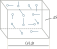
\includegraphics[scale=1.0]{figures/ch_11/fig_11_6.pdf}
		\caption[]{}
		\label{fig:11_6}
	\end{center}
	\vspace{-0.8cm}
\end{figure}

Let us also assume that all the molecules travel with the same speed equal to $\average{v}$. Therefore, during the time $\Delta t$, the wall element $\Delta S$ will be reached by all the molecules moving toward it that are inside a cylinder with the base $\Delta S$ and the altitude $\average{v}\Delta t$ (\fig{11_6}). The number of these molecules is $\Delta\nu=(n/6)\Delta S\average{v}\Delta t$. Accordingly, the number of collisions with a unit area in unit time will be
\begin{equation}\label{eq:11_24}
	\nu = \frac{1}{6}n\average{v}.
\end{equation}

\noindent
The expression obtained differs from \eqn{11_23} only in the value of the numerical factor ($1/6$ instead of $1/4$).

Retaining our assumption on the motion of the molecules in three mutually perpendicular directions, but negating the assumption on the molecules having identical speeds, we must separate from among the molecules in unit volume those $\deriv{n_v}$ molecules whose speed ranges from $v$ to $v+\deriv{v}$. The number of molecules having such speeds and reaching the area $\Delta S$ during the time $\Delta t$ is
\begin{equation}\label{eq:11_25}
	\deriv{\nu_v} = \frac{1}{6}v\Delta S \Delta t\,\deriv{n_v}.
\end{equation}

\noindent
We get the total number of collisions by integrating \eqn{11_25} with respect to speeds:
\begin{equation*}
	\Delta\nu = \int \deriv{\nu_v} = \frac{1}{6} \Delta S \Delta t \int_{0}^{\ab{v}{max}} v\,\deriv{n_v} = \frac{1}{6}n \average{v}\Delta S \Delta t.
\end{equation*}

\noindent
Finally, dividing $\Delta\nu$ by $\Delta S$ and $\Delta t$, we get \eqn{11_24}. Thus, our assumption that the molecules have identical speeds does not affect the result obtained for the number of collisions of the molecules with the wall. As we shall see in the following section, however, this assumption changes the result of pressure calculations.

\section{Pressure of a Gas on a Wall}\label{sec:11_4}

The walls of a vessel containing a gas are continuously bombarded by its molecules. The result is that the wall element $\Delta S$ receives a momentum during one second that equals the force acting on this element. The ratio of this force to the area $\Delta S$ gives the pressure exerted by the gas on the walls of the vessel. The pressure of the gas on different portions of the vessel walls is the same owing to the chaotic nature of motion of the molecules (naturally, provided that the gas is in an equilibrium state).

\begin{figure}[t]
	\begin{center}
		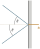
\includegraphics[scale=1.0]{figures/ch_11/fig_11_7.pdf}
		\caption[]{}
		\label{fig:11_7}
	\end{center}
	\vspace{-0.8cm}
\end{figure}

If we assume that the molecules rebound from a wall according to the law of mirror reflection ($\ab{\theta}{ref}=\ab{\theta}{inc}$) and the magnitude of the velocity of a molecule does not change\footnote{The interaction of the molecules with the walls of the vessel is actually of a more complicated nature (see Sec.~\ref{sec:16_6}), and our assumptions hold only on the average for a great number of collisions.}, then the momentum imparted by a molecule to the wall upon colliding with it will be $2mv\cos\theta$ (\fig{11_7}), where $m$ is the mass of a molecule. This momentum is directed along a normal to the area. Each of the $\deriv{\nu_{v,\theta,\varphi}}$ molecules [see \eqn{11_19}] imparts a momentum of $2mv\cos\theta$ to the wall, and all these molecules impart a momentum of
\begin{equation*}
	\deriv{K_{v,\theta,\varphi}} = 2mv\cos\theta\,\deriv{\nu_{v,\theta,\varphi}} = \deriv{N_v} \frac{\deriv{\Omega_{\theta,\varphi}}}{4\pi}\frac{2mv^2\cos^2\theta\Delta S\Delta t}{V}.
\end{equation*}

\noindent
(We have used the symbol $K$ for the momentum instead of the previously used symbol $p$ to avoid confusion---the latter symbol stands for pressure here.)

Summation of the expression obtained by directions within the limits of the solid angle $2\pi$ (corresponding to changes in $\theta$ from $0$ to $\pi/2$ and changes in $\varphi$ from $0$ to $2\pi$) gives the momentum imparted by the molecules whose velocities have magnitudes ranging from $v$ to $v+\deriv{v}$:
\begin{equation*}
	\deriv{K_v} = \deriv{N_v} \frac{2mv^2\Delta S\Delta t}{4\pi V} \int_{0}^{\pi/2}\cos^2\theta\sin\theta\,\deriv{\theta} \int_{0}^{2\pi}\deriv{\varphi}
\end{equation*}

\noindent
[we have introduced \eqn{11_15} for $\deriv{\Omega}$]. Integration with respect to $\deriv{\varphi}$ yields $2\pi$, and the integral with respect to $\deriv{\theta}$ is $1/3$. Hence,
\begin{equation*}
	\deriv{K_v} = \deriv{N_v} \frac{mv^2\Delta t}{3V}.
\end{equation*}

\noindent
Integrating this expression with respect to velocities from $0$ to $\ab{v}{max}$ we get the total momentum imparted to the area $\Delta S$ during the time $\Delta t$:
\begin{equation}\label{eq:11_26}
	\Delta K = \frac{m\Delta S\Delta t}{3V} \int_{0}^{\ab{v}{max}} v^2\,\deriv{N_v}.
\end{equation}

The expression
\begin{equation*}
	\frac{1}{N}\int_{0}^{\ab{v}{max}} v^2\,\deriv{N_v}
\end{equation*}

\noindent
is the mean value of the square of the velocity of the molecules. Substituting the product $N\average{v^2}$ for the integral in \eqn{11_26}, we find that
\begin{equation*}
	\Delta K = \frac{m\Delta S\Delta t}{3V} N \average{v^2} = \frac{1}{3} nm \average{v^2} \Delta S\Delta t
\end{equation*}

\noindent
($n=N/V$ is the number of molecules in unit volume). Finally, dividing this expression by $\Delta S$ and $\Delta t$, we obtain the pressure of a gas on the walls of the vessel containing it:
\begin{equation}\label{eq:11_27}
	p = \frac{1}{3} nm \average{v^2} = \frac{2}{3} n \frac{m\average{v^2}}{2}.
\end{equation}

We have assumed that all the molecules have the same mass. We can therefore put it inside the sign of the mean quantity. As a result, \eqn{11_27} acquires the form
\begin{equation}\label{eq:11_28}
	p = \frac{2}{3} n \average{\frac{mv^2}{2}} = \frac{2}{3}n\average{\ab{\varepsilon}{tr}}
\end{equation}

\noindent
where $\average{\ab{\varepsilon}{tr}}$ is the mean value of the kinetic energy of translation of the molecules.

Let us obtain an expression for the pressure proceeding from the simplified notions that led us to \eqn{11_24}. According to these notions, each molecule imparts a momentum of $2m\average{v}$ to the wall it collides with. Multiplying this momentum by the number of collisions [see \eqn{11_24}], we get the momentum imparted to a unit area in unit time, \ie, the pressure. We thus obtain the equation
\begin{equation}\label{eq:11_29}
	p = \frac{1}{6} n \average{v} \times 2m\average{v} = \frac{1}{3}nm\average{v}^2.
\end{equation}

\noindent
This equation differs from \eqn{11_27} in that it contains the square of the mean velocity $\average{v}^2$ instead of the mean square of the velocity $\average{v^2}$. We shall see on a later page (in Sec.~\ref{sec:11_5}) that these two quantities differ from each other, \ie, $\average{v^2}\neq\average{v}^2$.

In a more accurate calculation, we must multiply the number of molecules determined according to \eqn{11_25} by $2mv$ and then summate over all the $v$'s. As a result, we get the momentum imparted to the area $\Delta S$ during the time $\Delta t$:
\begin{align*}
	\Delta K &= \int_{0}^{\ab{v}{max}} \frac{1}{6}\,\deriv{n_v}\Delta S\Delta t \times 2mv = \frac{1}{3}m \Delta S\Delta t \int_{0}^{\ab{v}{max}} v^2\,\deriv{n_v}\\
	&= \frac{1}{3}nm\average{v^2} \Delta S\Delta t.
\end{align*}

\noindent
Dividing this equation by $\Delta S$ and $\Delta t$, we get \eqn{11_27} for the pressure. Thus, on the basis of our simplified notion of the molecules travelling in three mutually perpendicular directions, we have obtained an exact expression for the pressure. The explanation is that this simplification leads on the one hand to diminishing of the number of collisions of the molecules with the wall [$n\average{v}/6$ instead of $n\average{v}/4$, see Eqs.~\eqref{eq:11_23} and~\eqref{eq:11_24}], and on the other to overstating of the momentum transmitted to the wall in each collision. In our simplified derivation, we assumed that the wall receives a momentum of $2mv$ upon each collision. Actually, however, the magnitude of the momentum imparted to the wall depends on the angle $\theta$, and as a result the mean momentum imparted in one collision is $4mv/3$. In the long run, both inaccuracies mutually compensate each other and, notwithstanding the simplified nature of our derivation, we obtain an exact expression for the pressure.

\section{Mean Energy of Molecules}\label{sec:11_5}

Let us write \eqn{11_28} for the pressure obtained in the preceding section and the equation of state~\eqref{eq:10_21} of an ideal gas next to each other:
\begin{equation*}
	p = \frac{2}{3}n\average{\ab{\varepsilon}{tr}},\quad p = nkT.
\end{equation*}

\noindent
A comparison of these equations shows that
\begin{equation}\label{eq:11_30}
	\average{\ab{\varepsilon}{tr}} = \frac{3}{2}kT.
\end{equation}

\noindent
We have thus arrived at an important conclusion: \textbf{the absolute temperature is a quantity proportional to the mean energy of translation of molecules}. Only gas molecules have translation. For liquids and solids, the mean energy of the molecules is proportional to the absolute temperature only when the motion of the molecules can be treated classically. In the quantum region, the mean energy of the molecules stops being proportional to the absolute temperature.

Equation~\eqref{eq:11_30} is remarkable in that the mean energy is found to depend only on the temperature and is independent of the mass of a molecule.

Since $\average{\ab{\varepsilon}{tr}}=\average{mv^2/2}=(m/2)\average{v^2}$ it follows from \eqn{11_30} that
\begin{equation}\label{eq:11_31}
	\average{v^2} = \frac{3kT}{2m}.
\end{equation}

\noindent
Representing $\average{v^2}$ in the form of the sum of the squares of the velocity components, we can write:
\begin{equation*}
	\average{v_x^2} = \average{v_y^2} = \average{v_z^2}.
\end{equation*}

\noindent
Taking this into account, we find that
\begin{equation}\label{eq:11_32}
	\average{v_x^2} = \frac{1}{3}\average{v^2} = \frac{kT}{m}.
\end{equation}

Equation~\eqref{eq:11_30} determines the energy of only the translation of a molecule. In addition to translation, however, rotation of a molecule and vibrations of the atoms in the molecule are possible. Both these kinds of motion are associated with a certain store of energy. The latter can be determined by the theorem on the equal distribution of the energy by the degrees of freedom of a molecule established by statistical physics.

\textit{The number of degrees of freedom of a mechanical system is defined as the number of independent quantities by means of which we can set the position of the system}. Thus, the position of a point particle in space is determined completely by setting the values of three of its coordinates (for example, the Cartesian coordinates $x, y, z$, or the spherical coordinates $r, \theta, \varphi$, etc.). Accordingly, a point particle has three degrees of freedom.

\begin{figure}[t]
	\begin{center}
		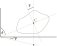
\includegraphics[scale=1.0]{figures/ch_11/fig_11_8.pdf}
		\caption[]{}
		\label{fig:11_8}
	\end{center}
	\vspace{-0.8cm}
\end{figure}

The position of a perfectly rigid body can be determined by setting three coordinates of its centre of mass $(x, y, z)$, the two angles $\theta$ and $\varphi$ indicating the direction of an axis associated with the body and passing through its centre of mass (\fig{11_8}), and, finally, the angle $\psi$ determining the direction of a second axis associated with the body and perpendicular to the first one. Hence, a perfectly rigid body has six degrees of freedom. A change in the coordinates of the centre of mass with the angles $\theta$, $\varphi$, and $\psi$ remaining constant is due to translation of a rigid body. Therefore, the relevant degrees of freedom are called \textbf{translational}. A change in any of the angles $\theta, \varphi, \psi$ with an unchanging position of the centre of mass is due to rotation of a body, and in this connection the corresponding degrees of freedom are called \textbf{rotational}. Hence, of the six degrees of freedom of a perfectly rigid body, three are translational and three rotational.

A system of $N$ point particles between which there are no rigid constraints has $3N$ degrees of freedom (the position of each of the $N$ particles must be set by three coordinates). Any rigid constraint establishing an unchanging mutual arrangement of two particles reduces the number of degrees of freedom by one. For example, if a system consists of two point particles with a constant distance $l$ between them (\fig{11_9}), then the number of degrees of freedom of the system is five. Indeed, in this case, the following relation holds between the coordinates of the particles:
\begin{equation}\label{eq:11_33}
	(x_2 - x_1)^2 + (y_2 - y_1)^2 + (z_2 - z_1)^2 = l^2
\end{equation}

\noindent
owing to which the coordinates will not be independent: it is sufficient to set any five coordinates, and the sixth one will be determined by condition~\eqref{eq:11_33}. To classify these five degrees of freedom, we shall note that the position of a system formed by two rigidly connected point particles can be determined as follows: we can set the three coordinates of the centre of mass of the system (\fig{11_10}) and the two angles $\theta$ and $\varphi$ that determine the direction in space of the axis of the system (\ie, the straight line passing through both points). It thus follows that three degrees of freedom will be translational and two rotational. The latter correspond to rotation about two mutually perpendicular axes $0'0'$ and $0''0''$ that are at right angles to axis $00$ of the system (\fig{11_11}). Rotation about axis $00$ is deprived of meaning for point particles.

\begin{figure}[t]
	\begin{minipage}[t]{0.5\linewidth}
		\begin{center}
			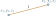
\includegraphics[scale=1.0]{figures/ch_11/fig_11_9.pdf}
			\caption[]{}
			\label{fig:11_9}
		\end{center}
	\end{minipage}
	\hspace{-0.05cm}
	\begin{minipage}[t]{0.5\linewidth}
		\begin{center}
			\includegraphics[scale=1.0]{figures/ch_11/fig_11_10.pdf}
			\caption[]{}
			\label{fig:11_10}
		\end{center}
	\end{minipage}
%	\vspace{-0.4cm}
\end{figure}

\begin{figure}[t]
	\begin{minipage}[t]{0.5\linewidth}
		\begin{center}
			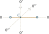
\includegraphics[scale=1.0]{figures/ch_11/fig_11_11.pdf}
			\caption[]{}
			\label{fig:11_11}
		\end{center}
	\end{minipage}
	\hspace{-0.05cm}
	\begin{minipage}[t]{0.5\linewidth}
		\begin{center}
			\includegraphics[scale=1.0]{figures/ch_11/fig_11_12.pdf}
			\caption[]{}
			\label{fig:11_12}
		\end{center}
	\end{minipage}
	\vspace{-0.4cm}
\end{figure}

If two point particles are connected by an elastic constraint instead of a rigid one (\ie, so that any change in the equilibrium distance $r_0$ between the particles results in the setting up of forces tending to establish the initial distance between the particles), then the number of degrees of freedom will be six. The position of the system in this case can be determined by setting the three coordinates of the centre of mass (\fig{11_12}), the two angles $\theta$ and $\varphi$, and the distance $r$ between the particles. Changes in $r$ correspond to vibrations in the system, consequently this degree of freedom is called \textbf{vibrational}. Thus, the system considered has three translational, two rotational, and one vibrational degree of freedom.

Let us consider a system consisting of $N$ point particles elastically connected to one another. Such a system has $3N$ degrees of freedom. The particles have an equilibrium configuration corresponding to a minimum potential energy of the system. The equilibrium configuration is characterized by quite definite mutual distances between the particles. If the particles are brought out of their positions corresponding to equilibrium configuration, vibrations appear in the system. The position of the system can be determined by setting the position of the equilibrium configuration and the quantities characterizing the displacements of the particles from their equilibrium positions. The latter quantities correspond to the vibrational degrees of freedom.

The position of equilibrium configuration, like that of a perfectly rigid body, is determined by six quantities which three translational and three rotational degrees of freedom correspond to. The number of vibrational degrees of freedom is thus $3N-6$\footnote{It is assumed that the equilibrium positions of the particles are not on one straight line. Otherwise there will be only two rotational degrees of freedom, and $3N-5$ vibrational ones. We treated this case in dealing with a system consisting of two particles.}.

Experiments on measuring the heat capacity of gases have shown that atoms must be treated as point particles in determining the number of degrees of freedom of a molecule. Consequently, three translational degrees of freedom should be ascribed to a monatomic molecule. The degrees of freedom ascribed to a diatomic molecule depend on the nature of the bond between the atoms. They include either three translational and two rotational degrees of freedom (with a rigid bond), or, apart from these five, another vibrational degree of freedom (with an elastic bond). A triatomic molecule with rigid bonds has three translational and three rotational degrees of freedom, etc.

We must note that no matter how many degrees of freedom a molecule has, three of them are translational. Since none of the translational degrees of freedom of a molecule has priority over the other two, an identical energy should fall to each of them on an average. This energy is one-third of the value given by \eqn{11_30}, \ie, $kT/2$.

The \textbf{equipartition principle} is derived in classical statistical physics\footnote{This derivation is beyond the scope of a course in general physics.}. It states that \textit{an identical kinetic energy equal to $kT/2$ resides on the average in any degree of freedom}.

According to this principle, the mean energy of one molecule $\average{\varepsilon}$ will be the greater (at the same temperature), the more complex is the molecule and the more degrees of freedom it has. In determining $\average{\varepsilon}$, we must take into account that a vibrational degree of freedom must have an energy capacity that is twice the value for a translational or rotational one. The explanation is that translation and rotation of a molecule are associated with the presence of only kinetic energy, whereas vibration is associated with the presence of both kinetic and potential energy; for a harmonic oscillator, the mean value of the kinetic and the potential energy is the same. Hence, two halves of $kT$ must reside in each vibrational degree of freedom---one in the form of kinetic energy and one in the form of potential energy.

Thus, the mean energy of a molecule should be
\begin{equation}\label{eq:11_34}
	\average{\varepsilon} = \frac{i}{2}kT
\end{equation}

\noindent
where $i$ is the sum of the number of translational ($\ab{n}{tr}$), the number of rotational ($\ab{n}{rot}$), and the double number of vibrational ($\ab{n}{vib}$) degrees of freedom of a molecule:
\vspace{-12pt}
\begin{equation}\label{eq:11_35}
	i = \ab{n}{tr} + \ab{n}{rot} + 2\ab{n}{vib}.
\end{equation}

\noindent
For molecules with a rigid bond between their atoms, $i$ coincides with the number of degrees of freedom of a molecule.

Molecules of an ideal gas do not interact with one another. We can therefore find the internal energy of one mole of an ideal gas by multiplying the Avogadro constant by the mean energy of one molecule:
\begin{equation}\label{eq:11_36}
	\ab{U}{m} = \ab{N}{A}\average{\varepsilon} = \frac{i}{2}\ab{N}{A} kT = \frac{i}{2}RT.
\end{equation}

\noindent
A comparison of this equation with \eqn{10_28} shows that
\begin{equation}\label{eq:11_37}
	C_V = \frac{i}{2}R.
\end{equation}

\noindent
With a view to \eqn{10_33}, we find that
\begin{equation}\label{eq:11_38}
	C_p = \left(\frac{i+2}{2}\right) R.
\end{equation}

\noindent
Hence,
\begin{equation}\label{eq:11_39}
	\gamma = \frac{C_p}{C_V} = \frac{i+2}{i}.
\end{equation}

\noindent
Thus, the quantity $\gamma$ is determined by the number and the nature of degrees of freedom of a molecule.

Table~\ref{table:11_1} gives the values of $C_V$, $C_p$, and $\gamma$ obtained for different species of molecules by Eqs.~\eqref{eq:11_37}, \eqref{eq:11_38}, and~\eqref{eq:11_39}. Table~\ref{table:11_2} compares the theoretical results with experimental data. The theoretical values have been obtained (except for the case indicated in the footnote to the table) on the assumption that the molecules are rigid; the experimental values have been obtained for temperatures close to room temperature.

\begin{table}[!b]
	\renewcommand{\arraystretch}{1.2}
	\caption{ }
	\vspace{-0.6cm}
	\label{table:11_1}
	\begin{center}\resizebox{0.82\linewidth}{!}{
			\begin{tabular}{l p{1.59cm} ccccccc}
				\toprule[1pt]
				\multirow{2}{*}{\textbf{Molecule}} & \textbf{Nature of Molecule} & \multirow{2}{*}{$\ab{n}{tr}$} & \multirow{2}{*}{$\ab{n}{rot}$} & \multirow{2}{*}{$\ab{n}{vib}$} & \multirow{2}{*}{$i$} & \multirow{2}{*}{$C_V$} & \multirow{2}{*}{$C_p$} & \multirow{2}{*}{$\gamma$}\\
				\midrule[0.5pt]\midrule[0.5pt]
				Monoatomic & --- & $3$ & --- & --- & $3$ & $\frac{3}{2}R$ & $\frac{5}{2}R$ & $1.67$\\
				Diatomic & Rigid & $3$ & $2$ & --- & $5$ & $\frac{5}{2}R$ & $\frac{7}{2}R$ & $1.40$\\
				Diatomic & Elastic & $3$ & $2$ & $1$ & $7$ & $\frac{7}{2}R$ & $\frac{9}{2}R$ & $1.29$\\
				$\geqslant 3$ atoms & Rigid & $3$ & $3$ & --- & $6$ & $\frac{6}{2}R$ & $\frac{8}{2}R$ & $1.33$\\
				\bottomrule[1pt]
			\end{tabular}
	}\end{center}
\end{table}

\begin{table}[!b]
	\renewcommand{\arraystretch}{1.2}
	\caption{ }
	\vspace{-0.6cm}
	\label{table:11_2}
	\begin{center}\resizebox{0.98\linewidth}{!}{
			\begin{threeparttable}[b]
			\begin{tabular}{lccccccc}
				\toprule[1pt]
				\multirow{2}{*}{\textbf{Gas}} & \multirow{2}{2.3cm}{\textbf{No. of atoms in molecule}} & \multicolumn{2}{c}{$C_V\times\num{e-3}$} &
				\multicolumn{2}{c}{$C_p\times\num{e-3}$} & \multicolumn{2}{c}{$\gamma$} \\
				& & Theor. & Exp. & Theor. & Exp. & Theor. & Exp.\\
				\midrule[0.5pt]\midrule[0.5pt]
				Helium (He)&$1$&$12.5$&$12.5$&$20.8$&$20.9$&$1.67$&$1.67$\\
				Oxygen (\ce{O2})&$2$&$20.8$&$20.9$&$29.1$&$28.9$&$1.40$&$1.40$\\
				Carbon monoxide (CO)&$2$&$20.8$&$21.0$&$29.1$&$29.3$&$1.40$&$1.40$\\
				Water vapour (\ce{H2O})&$3$&$25.0$&$27.8$&$33.2$&$36.2$&$1.33$&$1.31$\\
				& & $33.2$\tnote{${\dagger}$} & & $41.5$\tnote{${\dagger}$} & & $1.25$\tnote{${\dagger}$} & \\
				\bottomrule[1pt]
			\end{tabular}
		\begin{tablenotes}
			\item [${\dagger}$] For $i=8$, \ie, assuming that there is additionally one vibrational degree of freedom.
		\end{tablenotes}
	\end{threeparttable}
	}\end{center}
\end{table}

It should seem to follow from Table~\ref{table:11_2} that agreement between theory and experiments is quite satisfactory, at any rate for monatomic and diatomic molecules. Actually, however, matters are different. According to the theory we have considered, the heat capacities of gases ought to be integral multiples of $R/2$ because the number of degrees of freedom can only be integral. Therefore, even small deviations of $C_V$ and $C_p$ from values that are multiples of $R/2$ have fundamental significance. Examination of the table shows that such deviations, exceeding the possible errors of measurements, are encountered.

\begin{figure}[t]
	\begin{center}
		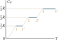
\includegraphics[scale=1.0]{figures/ch_11/fig_11_13.pdf}
		\caption[]{}
		\label{fig:11_13}
	\end{center}
	\vspace{-0.8cm}
\end{figure}

The discrepancies between theory and experiments become especially striking if we turn to the temperature dependence of the heat capacity. Figure~\ref{fig:11_13} shows a curve of the temperature dependence of the molar heat capacity $C_V$ obtained experimentally for hydrogen. The heat capacity should be independent of the temperature according to theory. A glance at the figure shows that this holds only within the limits of separate temperature intervals, and that within different intervals the heat capacity has values corresponding to different numbers of degrees of freedom of a molecule. Thus, on portion $1$-$1'$, we have $C_V=3R/2$. This signifies that a molecule behaves like a system having only translational degrees of freedom. On portion $2$-$2'$, we have $C_V=5R/2$. Hence, at temperatures corresponding to this portion of the curve, in addition to the three translational degrees of freedom manifesting themselves at lower temperatures, two rotational ones appear in a molecule. Finally, at sufficiently high temperatures, $C_V$ becomes equal to $7R/2$, which points to the presence of vibrations of a molecule at these temperatures. Between these intervals, the heat capacity monotonously grows with increasing temperature, \ie, corresponds, as it were, to a fractional varying number of degrees of freedom.

Thus, the number of degrees of freedom of a molecule manifesting itself in the heat capacity depends on the temperature. At low temperatures, only translation of the molecules is observed. At higher temperatures, rotation of the molecules is observed in addition to translation. And, finally, at still higher temperatures, vibrations of the molecules are also added to the first two kinds of motion. As indicated by the monotonous nature of the heat capacity curve, here not all the molecules at a time are involved in rotation, and then in vibration. First rotation, for example, begins to be observed only in a small fraction of the molecules. This fraction grows with elevation of the temperature, and in the long run when a definite temperature is reached, virtually all the molecules will be involved in rotation.

Matters are similar for vibration of the molecules. This behaviour of the heat capacity is explained by quantum mechanics. The quantum theory has established that the energy of rotation and vibration of molecules is quantized. This signifies that the energy of rotation and that of vibration of a molecule cannot have any values, but only discrete ones (\ie, values differing from one another by a finite amount). Consequently, the energy associated with these kinds of motion can change only in jumps. Such restrictions do not exist for the energy of translation.

The intervals between separate allowed values of the energy (or, in accordance with the adopted terminology, between energy levels) are about an order greater for vibration than for rotation. A simplified diagram of the rotational and vibrational levels of a diatomic molecule is given in \fig{11_14}. (The distances between the rotational levels are actually not the same, but this is of no significance for the question being considered.)

\begin{figure}[t]
	\begin{center}
		\includegraphics[scale=1.0]{figures/ch_11/fig_11_14.pdf}
		\caption[]{}
		\label{fig:11_14}
	\end{center}
	\vspace{-0.8cm}
\end{figure}

We noted in Sec.~\ref{sec:11_2} that the velocities of molecules are mainly grouped near a most probable value. Accordingly, the predominating part of molecules have energies close to the mean value $\average{\varepsilon}$, and only a small part of the molecules have energies considerably exceeding $\average{\varepsilon}$. Hence, for an appreciable part of the molecules to be involved in rotation or vibration, their mean energy must be sufficiently high in comparison with the distance between the allowed levels of the relevant energy.

Let us take such a low temperature that the mean energy of a molecule $\average{\varepsilon}$ is considerably lower than the first allowed value of the rotational energy (see the bottom dash line in \fig{11_14}). Now only an insignificant part of all the molecules will be involved in rotation, so that the molecules of the gas will virtually have only translation. Small changes in the temperature will result in changes only in the energy of translation, and the heat capacity of the gas will accordingly be $3R/2$ (see $1$-$1'$ on the curve depicted in \fig{11_13}).

Elevation of the temperature is attended by an increase in $\average{\varepsilon}$ so that a constantly growing part of the molecules will be involved in rotation. Portion $1'$-$2$ of the curve in \fig{11_13} corresponds to this process.

After all the molecules begin to participate in rotation, the horizontal portion $2$-$2'$ commences. At temperatures corresponding to it, the value of $\average{\varepsilon}$ is still considerably lower than the distance between the allowed levels of vibrational energy. As a result, vibration of the molecules will virtually be absent. With a further elevation of the temperature, the molecules will begin to vibrate in greater and greater numbers, which transition portion $2'$-$3$ on the heat capacity curve corresponds to. Finally, at a sufficiently high temperature, all the molecules will be involved in vibration, and the heat capacity will become equal to $7R/2$.

The classical theory of heat capacity is thus approximately correct only for separate temperature intervals. A different number of degrees of freedom of a molecule corresponds to each interval.

\section{The Maxwell Distribution}\label{sec:11_6}

We shall use the following procedure to find a way of quantitatively describing the distribution of molecules by velocity magnitudes. Let us take Cartesian coordinate axes in an imaginary space which we shall call $v$-space (velocity space). We shall lay off the values of $v_x, v_y, v_z$ of individual molecules along these axes (what we have in view are the velocity components along the axes $x, y, z$ taken in conventional space). Hence, a point in this $v$-space will correspond to the velocity of each molecule. Owing to collisions, the positions of the points will continuously change, but their density at each place will remain unchanged (we remind our reader that we are dealing with an equilibrium state of a gas).

Owing to all the directions of motion having equal rights, the arrangement of the points relative to the origin of coordinates will be spherically symmetrical. Hence, the density of the points in our $v$-space can depend only on the magnitude of the velocity $v$ (or on $\vec{v}^2$). Let us denote this density by $Nf(v)$ (here $N$ is the total number of molecules in the given mass of gas). Hence, the number of molecules whose velocity components are within the limits from $v_x$ to $v_x+\deriv{v_x}$, from $v_y$ to $v_y+\deriv{v_y}$, and from $v_z$ to $v_z+\deriv{v_z}$ can be written in the form
\begin{equation}\label{eq:11_40}
	\deriv{N_{v_x, v_y, v_z}} = Nf(v)\,\deriv{v_x}\,\deriv{v_y}\,\deriv{v_z}
\end{equation}

\noindent
(the product $\deriv{v_x}\,\deriv{v_y}\,\deriv{v_z}$ gives an element of volume in $v$-space).

\begin{figure}[t]
	\begin{center}
		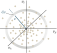
\includegraphics[scale=1.0]{figures/ch_11/fig_11_15.pdf}
		\caption[]{}
		\label{fig:11_15}
	\end{center}
	\vspace{-0.8cm}
\end{figure}

Points depicting velocities whose magnitude is confined within the limits from $v$ to $v+\deriv{v}$ are in the region between spheres of radii $v$ and $v+\deriv{v}$ (\fig{11_15}). The volume of this region is $4\pi v\,\deriv{v}$. Hence, the number of points in this region is determined by the expression
\begin{equation}\label{eq:11_41}
	\deriv{N_v} = Nf(v) 4\pi v\,\deriv{v}.
\end{equation}

\noindent
This equation gives the number of molecules with velocity magnitudes ranging from $v$ to $v+\deriv{v}$. Dividing it by $N$, we get the probability $\deriv{P_v}$ of the velocity of a molecule being within the limits from $v$ to $v+\deriv{v}$:
\begin{equation}\label{eq:11_42}
	\deriv{P_v} = f(v) 4\pi v\,\deriv{v}.
\end{equation}

\noindent
By comparing this expression with \eqn{11_6}, we conclude that
\begin{equation}\label{eq:11_43}
	F(v) = f(v) 4\pi v^2
\end{equation}

\noindent
plays the part of a distribution or partition function of the molecules of a gas by velocities.

The form of the function~\eqref{eq:11_43} was established theoretically in 1860 by James Maxwell (1831-1879). We approximately follow his reasoning in the derivation of the law of distribution of gas molecules by velocities set out below.

According to \eqn{11_6}, the probability of the velocity component $v_x$ of a molecule having a value within the limits from $v_x$ to $v_x+\deriv{v_x}$ can be written in the form
\begin{equation}\label{eq:11_44}
	\deriv{P_{v_x}} = \varphi(x)\,\deriv{v_x}
\end{equation}

\noindent
where $\varphi(x)$ is a distribution function. The similar probabilities for the other two components are determined by the equations
\begin{align}
	\deriv{P_{v_y}} &= \varphi(y)\,\deriv{v_y}, \label{eq:11_45}\\
	\deriv{P_{v_z}} &= \varphi(z)\,\deriv{v_z}. \label{eq:11_46}
\end{align}

\noindent
Owing to all directions of motion having equal rights, the analytical form of the functions $\varphi(v_x)$, $\varphi(v_y)$, and $\varphi(v_z)$ must be identical. These functions differ only in the designation of the argument.

Maxwell assumed that the probability of one of the components, for instance $v_x$, having different values does not depend on the values of the other two components (in our case $v_y$ and $v_z$)\footnote{This assumption can be proved very strictly, but the proof is beyond the cope of our course.}. This signifies that the events consisting in that $v_x$ of a molecule is within the limits from $v_x$ to $v_x+\deriv{v_x}$, $v_y$ of the same molecule is within the limits from $v_y$ to $v_y+\deriv{v_y}$, and, finally, $v_z$ of the same molecule is within the limits from $v_z$ to $v_z+\deriv{v_z}$, are statistically independent. Therefore the probability that the velocity components of a molecule have values within the limits from $v_X, v_y, v_z$ to $v_x+\deriv{v_x}, v_y+\deriv{v_y}, v_z+\deriv{v_z}$ equals the product of the probabilities given by Eqs.~\eqref{eq:11_44}-\eqref{eq:11_46}:
\begin{equation}\label{eq:11_47}
	\deriv{P_{v_x, v_y, v_z}} = \varphi(v_x)\varphi(v_y)\varphi(v_z)\,\deriv{v_x}\,\deriv{v_y}\,\deriv{v_z}
\end{equation}

\noindent
[see \eqn{11_4}]. At the same time, according to \eqn{11_40}, this probability can be written in the form
\begin{equation}\label{eq:11_48}
	\deriv{P_{v_x, v_y, v_z}} = f(v)\,\deriv{v_x}\,\deriv{v_y}\,\deriv{v_z}.
\end{equation}

A comparison of Eqs.~\eqref{eq:11_47} and~\eqref{eq:11_48} shows that
\begin{equation}\label{eq:11_49}
	f(v) = \varphi(v_x)\varphi(v_y)\varphi(v_z).
\end{equation}

\noindent
Taking logarithms of both sides of this equation, we get
\begin{equation*}
	\ln[f(v)] = \ln[\varphi(v_x)] + \ln[\varphi(y)] + \ln[\varphi(v_z)].
\end{equation*}

\noindent
Differentiation of this expression with respect to $v_x$ yields
\begin{equation}\label{eq:11_50}
	\frac{f'(v)}{f(v)}\diffpartial{v}{v_x} = \frac{\varphi'(v_x)}{\varphi(v_x)}.
\end{equation}

Since $v=\left(v_x^2+v_y^2+v_z^2\right)^{1/2}$, the partial derivative of $v$ with respect to $v_x$ is
\begin{equation*}
	\diffpartial{v}{v_x} = \frac{v_x}{\left(v_x^2+v_y^2+v_z^2\right)^{1/2}} = \frac{v_x}{v}.
\end{equation*}

\noindent
Introducing this value of the derivative into \eqn{11_50} and then transferring $v_x$ from the numerator of the left-hand side to the denominator of the right-hand one, we get the equation
\begin{equation}\label{eq:11_51}
	\frac{f'(v)}{f(v)}\frac{1}{v} = \frac{\varphi'(v_x)}{\varphi(v_x)} = \frac{1}{v_x}.
\end{equation}

\noindent
The right-hand side of this equation, and therefore its left-hand side, is independent of the variables $v_y$ and $v_z$. Consequently, it also cannot depend on $v_x$ [the quantities $v_x$, $v_y$, and $v_z$ in $f(v)$ are symmetrical, see \eqn{11_49}]. Thus, each of the expressions in the left-hand and right-hand sides of \eqn{11_51} equals a certain constant which we shall denote by $-\alpha$ (we shall see later that this constant is less than zero, \ie, $\alpha>0$).

Hence,
\begin{equation*}
	\frac{\varphi'(v_x)}{\varphi(v_x)}\frac{1}{v_x} = -\alpha,\quad \text{or}\quad \frac{\varphi'(v_x)}{\varphi(v_x)} = -\alpha v_x.
\end{equation*}

\noindent
Integration yields
\begin{equation*}
	\ln[\varphi(v_x)] = -\frac{\alpha v_x^2}{2} + \ln{A}
\end{equation*}

\noindent
where $A$ is a constant. Thus,
\begin{equation}\label{eq:11_52}
	\varphi(v_x) = A \exp\left(-\frac{\alpha v_x^2}{2}\right).
\end{equation}

\noindent
Similarly,
\begin{equation*}
	\varphi(v_y) = A \exp\left(-\frac{\alpha v_y^2}{2}\right),\quad \varphi(v_z) = A \exp\left(-\frac{\alpha v_z^2}{2}\right).
\end{equation*}

\noindent
Multiplication of these functions yields
\begin{equation}\label{eq:11_53}
	f(v) = A^3 \exp\left[-\frac{\alpha}{2}\left(v_x^2+v_y^2+v_z^2\right)\right] = A^3 \exp\left(-\frac{\alpha v^2}{2}\right).
\end{equation}

It can be seen from the form of functions~\eqref{eq:11_52} and~\eqref{eq:11_53} that the constant a must be greater than zero. If it were negative, these functions would grow without restriction with increasing $v$.

The constant $A$ is found from the normalization condition~\eqref{eq:11_7}. According to this condition,
\begin{equation}\label{eq:11_54}
	A \int_{-\infty}^{+\infty}  \exp\left(-\frac{\alpha v_x^2}{2}\right)\,\deriv{v_x} = 1.
\end{equation}

\noindent
We pointed out in Sec.~\ref{sec:11_2} that the values of $v$ (and, consequently, $v_x$ too) cannot exceed a certain very great, but finite value $\ab{v}{max}$. At the same time, we have taken $-\infty$ and $+\infty$ as the integration limits. This extension of the integration limits does not introduce an appreciable error. The integrand diminishes with increasing $v_x$ so rapidly that at sufficiently great values of $v_x$ it does not virtually differ from zero. Therefore, the contribution of the integration paths from $\ab{v}{max}$ to $\infty$ and from $-\ab{v}{max}$ to $-\infty$ is negligibly small.

The integral in \eqn{11_54} is a Poisson integral with $\beta=\alpha/2$ [see Appendix~\ref{sec:A_2}, \eqn{A_1}]. According to \eqn{A_3}, we have
\begin{equation}\label{eq:11_55}
	\int_{-\infty}^{+\infty}  \exp\left(-\frac{\alpha v_x^2}{2}\right)\,\deriv{v_x} = \left(\frac{\pi}{\alpha/2}\right)^{1/2} = \left(\frac{2\pi}{\alpha}\right)^{1/2}.
\end{equation}

\noindent
Introducing this value into \eqn{11_54}, we find that $A\sqrt{2\pi/\alpha}=1$. Hence,
\begin{equation}\label{eq:11_56}
	A = \left(\frac{\alpha}{2\pi}\right)^{1/2}.
\end{equation}

Using the found value of $A$ in Eqs.~\eqref{eq:11_52} and~\eqref{eq:11_53}, we arrive at the equations
\begin{align}
	\varphi(v_x) &= \left(\frac{\alpha}{2\pi}\right)^{1/2} \exp\left(-\frac{\alpha v_x^2}{2}\right),\label{eq:11_57}\\
	f(v) &= \left(\frac{\alpha}{2\pi}\right)^{3/2} \exp\left(-\frac{\alpha v^2}{2}\right).\label{eq:11_58}
\end{align}

To find the constant $\alpha$, we shall use the function~\eqref{eq:11_57} to calculate the value of $\average{v_x^2}$ and equate the expression obtained to the value of $kT/m$ found by calculating the pressure [see \eqn{11_31}]. In accordance with \eqn{11_11}
\begin{equation}\label{eq:11_59}
	\average{v_x^2} = \int_{-\infty}^{+\infty} v_x^2\varphi(v_x)\,\deriv{v_x} = \left(\frac{\alpha}{2\pi}\right)^{1/2} \int_{-\infty}^{+\infty} \exp\left(-\frac{\alpha v_x^2}{2}\right) v_x^2\,\deriv{v_x}.
\end{equation}

\noindent
According to \eqn{A_4}, we have
\begin{equation}\label{eq:11_60}
	\int_{-\infty}^{+\infty} \exp\left(-\frac{\alpha v_x^2}{2}\right) v_x^2\,\deriv{v_x} = \frac{1}{2}\left[\frac{\pi}{(\alpha/2)^3}\right]^{1/2} = \left(\frac{2\pi}{\alpha^3}\right)^{1/2}.
\end{equation}

Substituting for the integral in \eqn{11_59} its value from \eqn{11_60}, we find that
\begin{equation*}
	\average{v_x^2} = \left(\frac{\alpha}{2\pi}\right)^{1/2} \left(\frac{2\pi}{\alpha^3}\right)^{1/2} = \frac{1}{\alpha}.
\end{equation*}

\noindent
Comparison with \eqn{11_32} yields
\begin{equation}\label{eq:11_61}
	\alpha = \frac{m}{kT}.
\end{equation}

\noindent
The use of this value in Eqs.~\eqref{eq:11_57} and~\eqref{eq:11_58} leads to the final expressions for the distribution functions:
\begin{align}
	\varphi(v_x) &= \left(\frac{m}{2\pi kT}\right)^{1/2} \exp\left(-\frac{m v_x^2}{2kT}\right), \label{eq:11_62}\\
	f(v) &= \left(\frac{m}{2\pi kT}\right)^{3/2} \exp\left(-\frac{\alpha v^2}{2kT}\right).\label{eq:11_63}
\end{align}

It must be remembered that function~\eqref{eq:11_63} when multiplied by $N$ determines the density of the points depicting the velocities of the molecules in $v$-space. Multiplication of this function by $\deriv{v_x}\,\deriv{v_y}\,\deriv{v_z}$ gives the probability $\deriv{P_{v_x,v_y,v_z}}$ of the velocity components being within the limits from $v_X, v_y, v_z$ to $v_x+\deriv{v_x}, v_y+\deriv{v_y}, v_z+\deriv{v_z}$. Not only the magnitude of the velocity, but also its direction vary only within small limits determined by $\deriv{v_x}$, $\deriv{v_y}$, and $\deriv{v_z}$.
If we are interested only in the probability of the magnitude of the velocity regardless of the direction of motion of a molecule, \ie, $\deriv{P_v}$, then we must take the distribution function in the form of \eqn{11_43}. Multiplication of this function by $\deriv{v}$ gives the probability of the velocity of a molecule having the magnitude (with an arbitrary direction of motion) within the limits from $v$ to $v+\deriv{v}$.

According to Eqs.~\eqref{eq:11_43} and~\eqref{eq:11_63}, we have
\begin{equation}\label{eq:11_64}
	F(v) = \left(\frac{m}{2\pi kT}\right)^{3/2} \exp\left(-\frac{mv^2}{2kT}\right)\,4\pi v^2.
\end{equation}

\noindent
This function is characterized by the exponent containing the negative ratio between the kinetic energy of a molecule corresponding to the velocity $v$ being considered and $kT$, \ie, a quantity characterizing the mean energy of the molecules of a gas.

A graph of function~\eqref{eq:11_62} is shown in \fig{11_16}. It coincides with the Gaussian distribution of a random quantity.

\begin{figure}[t]
	\begin{minipage}[t]{0.5\linewidth}
		\begin{center}
			\includegraphics[scale=0.95]{figures/ch_11/fig_11_16.pdf}
			\caption[]{}
			\label{fig:11_16}
		\end{center}
	\end{minipage}
	\hspace{-0.05cm}
	\begin{minipage}[t]{0.5\linewidth}
		\begin{center}
			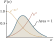
\includegraphics[scale=0.95]{figures/ch_11/fig_11_17.pdf}
			\caption[]{}
			\label{fig:11_17}
		\end{center}
	\end{minipage}
	\vspace{-0.7cm}
\end{figure}

A graph of function~\eqref{eq:11_64} is shown in \fig{11_17}. Since when $v$ increases, a factor of the kind $e^{-\alpha v^2}$ diminishes more rapidly than the factor $v^2$ grows, the function, which begins at zero (owing to $v^2$), reaches a peak and then asymptotically tends to zero. The area enveloped by the curve equals unity [compare with \eqn{11_7}]. Let us find the mean velocity of the molecules $\average{v}$ (we have in mind the arithmetical mean velocity). By analogy with \eqn{11_9}, we have
\begin{equation*}
	\average{v} = \int_{0}^{\infty} vF(v)\,\deriv{v} = \left(\frac{m}{2\pi kT}\right)^{3/2} 4\pi \int_{0}^{\infty} \exp\left(-\frac{mv^2}{2kT}\right)\,v^2\,\deriv{v}.
\end{equation*}

\noindent
By passing over to the variable $\zeta=v^2$ and integrating by parts, we arrive at the following result:
\begin{equation}\label{eq:11_65}
	\average{v} = \left(\frac{8kT}{\pi m}\right)^{1/2}.
\end{equation}

According to \eqn{11_11}
\begin{equation}\label{eq:11_66}
	\average{v^2} = \int_{0}^{\infty} v^2F(v)\,\deriv{v} = \left(\frac{m}{2\pi kT}\right)^{3/2} 4\pi \int_{0}^{\infty} \exp\left(-\frac{mv^2}{2kT}\right)\,v^4\,\deriv{v}.
\end{equation}

\noindent
From \eqn{A_6}, we get
\begin{equation*}
	\int_{0}^{\infty} \exp\left(-\frac{mv^2}{2kT}\right)\,v^4\,\deriv{v} = \frac{3}{8} \left(\frac{\pi}{(m/2kT)^5}\right)^{1/2} = \frac{3}{8\pi^2}\left(\frac{2\pi kT}{\pi}\right)^{5/2}.
\end{equation*}

\noindent
Introducing this value of the integral into \eqn{11_66}, we get for ($\average{v^2}$) the value $3kT/m$ that we already know [see \eqn{11_31}]. This is not surprising because when finding the value of $\alpha$ in \eqn{11_57} we proceeded from \eqn{11_32}, \ie, in essence from \eqn{11_31}.

The square root of $\average{v^2}$ is called the \textbf{mean square velocity}:
\begin{equation}\label{eq:11_67}
	\ab{v}{m. sq} = \sqrt{\average{v^2}} = \left(\frac{3kT}{m}\right)^{1/2}.
\end{equation}

The velocity corresponding to the maximum of $F(v)$ will be the most probable velocity. Taking the derivative of \eqn{11_64} with respect to $v$, omitting the constant factors and equating the expression obtained to zero, we arrive at the equation
\begin{equation*}
	\exp\left(-\frac{mv^2}{2kT}\right)\left[2 - \frac{mv^2}{kT}\right] v = 0.
\end{equation*}

\noindent
The values $v=0$ and $v=\infty$ satisfying this equation correspond to minima of $F(v)$. The value of $v$ making the expression in brackets vanish is the required most probable velocity $\ab{v}{prob}$:
\begin{equation}\label{eq:11_68}
	\ab{v}{prob} = \left(\frac{2kT}{m}\right)^{1/2}.
\end{equation}

By comparing Eqs.~\eqref{eq:11_65}, \eqref{eq:11_67}, and~\eqref{eq:11_67}, we find that
\begin{equation*}
	\ab{v}{prob}:\average{v}:\ab{v}{m. sq} = \sqrt{2}:\sqrt{8/\pi}:\sqrt{3} = 1 : 1.13 : 1.22.
\end{equation*}

\begin{figure}[t]
	\begin{minipage}[t]{0.5\linewidth}
		\begin{center}
			\includegraphics[scale=0.98]{figures/ch_11/fig_11_18.pdf}
			\caption[]{}
			\label{fig:11_18}
		\end{center}
	\end{minipage}
	\hspace{-0.05cm}
	\begin{minipage}[t]{0.5\linewidth}
		\begin{center}
			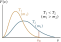
\includegraphics[scale=0.98]{figures/ch_11/fig_11_19.pdf}
			\caption[]{}
			\label{fig:11_19}
		\end{center}
	\end{minipage}
	\vspace{-0.4cm}
\end{figure}

\noindent
Figure~\ref{fig:11_18} illustrates this proportion.

Using \eqn{11_68} in~\eqref{eq:11_64}, we shall find the maximum value of the function $F(v)$:
\vspace{-12pt}
\begin{equation}\label{eq:11_69}
	F(\ab{v}{prob}) = \frac{4}{e}\left(\frac{m}{2kT}\right)^{1/2} \propto \left(\frac{m}{T}\right)^{1/2}.
\end{equation}

\noindent
It can be seen from Eqs.~\eqref{eq:11_68} and~\eqref{eq:11_69} that when the temperature grows (or the mass of a molecule diminishes), the peak of the curve moves to the right and becomes lower. The area confined by the curve, as we know, remains unchanged. Figure~\ref{fig:11_19} compares two distribution curves that can be interpreted either as relating to different temperatures $T_1$ and $T_2$ (with identical $m$), or as relating to different masses of the molecules $m_1$ and $m_2$ (with identical $T$).

The relative number of molecules whose velocity exceeds a certain value $v_0$ is determined by the expression
\begin{equation*}
	\int_{v_0}^{\infty} F(v)\,\deriv{v}.
\end{equation*}

\noindent
In \fig{11_19}, the part of the area confined by the curve that is, to the right of $v_0$ corresponds to this integral. It can be seen from the figure that the relative number of molecules having velocities exceeding $v_0$ greatly increases with elevation of the temperature.

Table~\ref{table:11_3} gives the relative number of molecules $\Delta N/N$ for different velocity intervals calculated with the aid of function~\eqref{eq:11_64}. Inspection of the table shows that the velocity of $70$\% of all the molecules differs from the most probable value by not over $50$\%. Only $0.04$\% of the molecules have a velocity exceeding $\ab{v}{prob}$ more than three times. And only one of $12000$ million molecules, on the average, has a velocity exceeding $5\ab{v}{prob}$.

\begin{table}[!b]
	\renewcommand{\arraystretch}{1.2}
	\caption{ }
	\vspace{-0.6cm}
	\label{table:11_3}
	\begin{center}\resizebox{0.28\linewidth}{!}{
			\begin{tabular}{cc}
				\toprule[1pt]
				$v/\ab{v}{prob}$ & $\Delta N/N$, \%\\
				\midrule[0.5pt]\midrule[0.5pt]
				$0.0$-$0.5$ & $8.10$\\
				$0.5$-$1.5$ & $70.7$\\
				$1.5$-$2.0$ & $16.6$\\
				$2.0$-$3.0$ & $4.60$\\
				$>3.0$ 		& $0.04$\\
				$>5.0$ 		& \num{8e-9}\\
				\bottomrule[1pt]
			\end{tabular}
 	}\end{center}
\end{table}

Let us assess the mean velocity of oxygen molecules. It is convenient to perform the calculations by replacing $k/m$ in \eqn{11_65} with the ratio $R/M$ equal to it. The expression for the mean velocity thus becomes
\begin{equation}\label{eq:11_70}
	\average{v} = \left(\frac{8RT}{\pi M}\right)^{1/2}.
\end{equation}

\noindent
The molecular mass of oxygen is $32$. Consequently, the mass of a mole $M=\SI{32e-3}{\kilo\gram\per\mole}$. Room temperature is about \SI{300}{\kelvin}. Introducing numerical values into \eqn{11_70}, we get
\begin{equation*}
	\average{v} = \left(\frac{8 \times 8.31 \times 300}{3.14 \times 32\times10^{-3}}\right)^{1/2} \approx \SI{500}{\metre\per\second}.
\end{equation*}

\noindent
Thus, each molecule of oxygen travels a path, on the average, of \SI{0.5}{\kilo\metre} in one second. Since a molecule collides very frequently with other molecules, this path consists of a great number of short straight lengths forming a broken line.

Hydrogen molecules have a mass that is $1/16$ that of an oxygen molecule. As a result, their velocity at the same temperature will be four times greater and will be almost \SI{2}{\kilo\metre\per\second} at room temperature.

If we have a mixture of gases in equilibrium, then the distribution~\eqref{eq:11_64} occurs within the limits of the molecules of each species with its own value of $m$. The heavier molecules will travel on the average with a lower velocity than the lighter ones.

On the basis of the distribution of molecules by velocities
\begin{equation}\label{eq:11_71}
	\deriv{N_v} = N \left(\frac{m}{2\pi kT}\right)^{3/2} \exp\left(-\frac{mv^2}{2kT}\right) 4\pi v^2,\deriv{v}
\end{equation}

\noindent
we can find the distribution of the molecules by their values of the kinetic energy of translation (we shall denote it by the symbol $\varepsilon$). For this purpose, we must pass over from a variable $v$ to a variable $\varepsilon$ equal to $mv^2/2$. Substituting $v=(2\varepsilon/m)^{1/2}$ and $\deriv{v}=(2m\varepsilon)^{-1/2}\,\deriv{\varepsilon}$ in \eqn{11_71}, we obtain
\begin{equation}\label{eq:11_72}
	\deriv{N_{\varepsilon}} = N \frac{2}{\sqrt{\pi}} (kT)^{-3/2} \exp\left(-\frac{\varepsilon}{kT}\right) \varepsilon^{1/2}\,\deriv{\varepsilon}
\end{equation}

\noindent
where $\deriv{N_{\varepsilon}}$ stands for the number of molecules whose kinetic energy of translation has values ranging from $\varepsilon$ to $\varepsilon+\deriv{\varepsilon}$.

The distribution of the molecules by values of $\varepsilon$ is thus characterized by the function
\begin{equation}\label{eq:11_73}
	f(\varepsilon) = A  \exp\left(-\frac{\varepsilon}{kT}\right) \varepsilon^{1/2}
\end{equation}

\noindent
where $A$ is a normalization factor equal to $(2/\sqrt{\pi}) (kT)^{-3/2}$.

\section{Experimental Verification of the Maxwell Distribution Law}\label{sec:11_7}

The first experimental determination of the velocities of molecules was conducted by 0. Stern in 1920. The apparatus he used for this purpose consisted of two coaxial cylinders (\fig{11_20}). A silver-coated platinum wire was made taut along the axis of the apparatus. When the wire was heated by passing an electric current through it, silver atoms evaporated from its surface. The velocities of the evaporated atoms corresponded to the temperature of the wire. The atoms travelled in radial directions after escaping from the wire. The inner cylinder had a narrow longitudinal slot through which a narrow beam of atoms (a molecular beam) passed outward. The entire apparatus was evacuated to prevent deviations of the silver atoms due to collisions with air molecules. After reaching the surface of the outer cylinder, the silver atoms settled on it and formed a layer having the shape of a narrow vertical stripe.

\begin{figure}[t]
	\begin{center}
		\includegraphics[scale=1.0]{figures/ch_11/fig_11_20.pdf}
		\caption[]{}
		\label{fig:11_20}
	\end{center}
	\vspace{-0.6cm}
\end{figure}

If the entire apparatus is brought into rotation, the trace left by the molecular beam will be displaced along the surface of the outer cylinder by the amount $\Delta s$ (see \fig{11_20}). This will occur because the apparatus manages to turn through the angle $\Delta\varphi$ while the silver atoms are flying through the space between the cylinders. As a result, a different part of the outer cylinder will be opposite the beam and it will be displaced relative to the initial trace $s_0$ by the amount $\Delta s$ equal to $R\Delta\varphi$ ($R$ is the radius of the outer cylinder). Considering the motion of the silver atoms in a rotating reference frame associated with the cylinders, the displacement of the trace can be explained by the action on the atoms of a Coriolis force equal to $2m(\vecprod{v}{\omega})$.

The distance $\Delta s$ between the original and the displaced stripes of silver can be related to the angular velocity of the cylinders $\omega$, the geometry of the apparatus, and the velocity of the atoms $v$. Denoting the flying time by $\Delta t$, we can write that
\begin{equation}\label{eq:11_74}
	\Delta s = \omega R\Delta t.
\end{equation}

\noindent
Since the radius of the inner cylinder is small in comparison with that of the outer cylinder $R$, the flying time can be assumed to equal
\begin{equation*}
	\Delta t = \frac{R}{v}.
\end{equation*}

\noindent
Using this expression in \eqn{11_74} and solving the resulting equation with respect to $v$, we get
\begin{equation*}
	v = \frac{\omega R^2}{\Delta s}.
\end{equation*}

The velocity of the atoms can be determined by measuring the displacement of the trace $\Delta s$ and the angular velocity of the apparatus. Complications are introduced, however, by the fact that owing to velocity distribution the atoms have different velocities. As a result, the displaced stripe will be blurred\footnote{The width of the stripe obtained with a stationary apparatus is determined only by the geometry of the apparatus, in particular by the	width of the slot through which the molecular beam emerges.}. By studying the profile of the trace (see \fig{11_20}), Stern found it possible to form an approximate notion of how the silver atoms are distributed by velocities.

The results of Stern's experiment confirmed the correctness of estimating the mean velocity of atoms that follows from the Maxwell distribution. This experiment, however, could give only very approximate information on the nature of the distribution itself.

\begin{figure}[t]
	\begin{center}
		\includegraphics[scale=1.0]{figures/ch_11/fig_11_21.pdf}
		\caption[]{}
		\label{fig:11_21}
	\end{center}
	\vspace{-0.7cm}
\end{figure}

The distribution law was verified more accurately in the experiment conducted by J. Lammert (1929). He passed a molecular beam through two rotating disks with radial slots displaced relative to each other through an angle $\varphi$ (\fig{11_21}). Only those of the molecules which pass through the slot in the first disk will fly through the second disk that arrive at it and encounter the slot in it. The faster molecules will reach the second disk too early, and the slower ones too late to pass through the slot. Thus, this apparatus makes it possible to separate molecules having a definite velocity from a beam (owing to the finite width of the slots, the apparatus separates molecules whose velocities are within a certain interval $\Delta v$). The mean velocity of the molecules separated by the apparatus can be found from the condition that the time $t_1$ during which the molecules cover the distance $l$ between the disks ($t_1=l/v$) must coincide with the time $t_2$ during which the disks rotate through the angle $\varphi$ (\ie, $t_1=\varphi/\omega$). Equating these two times, we get
\begin{equation*}
	v = \frac{\omega l}{\varphi}.
\end{equation*}

\noindent
By changing the angular velocity $\omega$ of the apparatus (or the angle $\varphi$ between the disks), we can separate molecules having different magnitudes of their velocity from the beam. By trapping these molecules during a definite time, we can find their relative number in the beam.

The results of Lammert's experiment and of other experiments undertaken for the same purpose completely agree with the distribution law established theoretically by Maxwell.

It must be noted that the distribution of molecules by velocities in a beam flying out through a hole in a vessel differs somewhat from the distribution in a closed vessel. Since the faster molecules will pass through the hole in a relatively greater number than the slower ones, the beam will be rich in the faster molecules. Because the number of molecules flying through the hole in unit time is proportional to $v$, the distribution in the beam will be characterized not by the function~\eqref{eq:11_64}, but by the function
\begin{equation*}
	F_1(v) = A_1 \exp\left(-\frac{mv^2}{2kT}\right) v^3
\end{equation*}

\noindent
where $A_1$ is a normalization factor. The most probable velocity in this case is $\ab{v}{prob}=\sqrt{3kT/m}$, and the mean velocity is $\average{v'}=\sqrt{9\pi kT/8m}$.

\section{The Boltzmann Distribution}\label{sec:11_8}

The barometric formula~\eqref{eq:10_71} obtained in Sec.~\ref{sec:10_14}, \ie,
\begin{equation*}
	p = p_0 \exp\left(-\frac{Mgh}{RT}\right)
\end{equation*}

\noindent
gives the dependence of the pressure on the altitude for an imaginary isothermal atmosphere. Let us replace $M/R$ in the exponent with the ratio $m/k$ equal to it ($m$ is the mass of a molecule, and $k$ is the Boltzmann constant). In addition, let us substitute $nkT$ for $p$ and $n_0kT$ for $p_0$ according to \eqn{10_21}. After cancelling $kT$ in both sides of the equation, we arrive at the formula
\begin{equation}\label{eq:11_75}
	n = n_0 \exp\left(-\frac{mgh}{kT}\right).
\end{equation}

\noindent
Here $n$ is the density of the molecules (\ie, their number in a unit volume) at the altitude $h$, and $n_0$ is the density of the molecules at the altitude $h_0=0$.

It can be seen from \eqn{11_75} that with lowering of the temperature, the number of particles at altitudes other than zero diminishes and vanishes at $T=0$ (\fig{11_22}). At absolute zero, all the molecules would be at the Earth's surface. At high temperatures, on the contrary, $n$ only slightly diminishes with increasing altitude so that the molecules are distributed by altitude almost uniformly.

\begin{figure}[t]
	\begin{center}
		\includegraphics[scale=1.0]{figures/ch_11/fig_11_22.pdf}
		\caption[]{}
		\label{fig:11_22}
	\end{center}
	\vspace{-0.5cm}
\end{figure}

This fact has a simple physical explanation. Each concrete distribution of the molecules by altitude sets in as a result of the action of two trends: (1) the attraction of the molecules to the Earth (characterized by the force $mg$) tends to arrange them on the Earth's surface, and (2) thermal motion (characterized by the quantity $kT$) tends to scatter the molecules uniformly over all the altitudes. The first trend prevails to a greater extent, the greater is $m$ and the smaller is $T$, and the molecules crowd together at the Earth's surface. In the limit at $T=0$, the thermal motion stops completely, and under the influence of the Earth's attraction the molecules occupy its surface. At high temperatures, thermal motion prevails, and the density of the molecules slowly diminishes with the altitude.

At different altitudes, a molecule has different stores of potential energy:
\begin{equation}\label{eq:11_76}
	\ab{\varepsilon}{p} = mgh.
\end{equation}

\noindent
Consequently, the distribution of the molecules by altitude is also their distribution by the values of the potential energy. In view of \eqn{11_76}, we can write \eqn{11_75} as follows:
\begin{equation}\label{eq:11_77}
	n = n_0 \exp\left(-\frac{\ab{\varepsilon}{p}}{kT}\right)
\end{equation}

\noindent
where $n$ is the density of the molecules at the spot in space where a molecule has the potential energy $\ab{\varepsilon}{p}$ and $n_0$ is the density of the molecules where the potential energy of a molecule vanishes.

Examination of \eqn{11_77} shows that the density of molecules per unit volume is greater where their potential energy is lower, and, conversely, their density is lower where their potential energy is greater.

According to \eqn{11_77}, the ratio of $n_1$ to $n_2$ at points where the potential energy of a molecule has the values $\ab{\varepsilon}{p,$1$}$ and $\ab{\varepsilon}{p,$2$}$ is
\begin{equation}\label{eq:11_78}
	\frac{n_1}{n_2} =  \exp\left[-\frac{\left(\ab{\varepsilon}{p,$1$} - \ab{\varepsilon}{p,$2$}\right)}{kT}\right].
\end{equation}

\noindent
L. Boltzmann proved that distribution~\eqref{eq:11_77} holds not only for the potential field of the Earth's gravitation, but also for any potential field of forces containing an assembly of any identical particles in a state of chaotic thermal motion. Accordingly, distribution~\eqref{eq:11_77} is called the \textbf{Boltzmann distribution}.

Whereas Maxwell's law gives the distribution of particles by values of their kinetic energy, Boltzmann's law gives their distribution by values of their potential energy. Both distributions are characterized by the presence of an exponential factor whose exponent is the ratio of the kinetic or, correspondingly, the potential energy of one molecule to the quantity determining the mean energy of thermal motion of a molecule.

According to \eqn{11_77}, the number of molecules contained in the volume $\deriv{V}=\deriv{x}\,\deriv{y}\,\deriv{z}$ at a point with the coordinates $x, y, z$ is
\begin{equation}\label{eq:11_79}
	\deriv{N_{x,y,z}} = n_0 \exp\left[-\frac{\ab{\varepsilon}{p}(x,y,z)}{kT}\right]\,\deriv{x}\,\deriv{y}\,\deriv{z}.
\end{equation}

\noindent
We have obtained another expression of the Boltzmann distribution law.

The Maxwell and Boltzmann distributions can be combined into the single \textbf{Maxwell-Boltzmann law} according to which the number of molecules whose velocity components are within the limits from $v_x, v_y, v_z$ to $v_x+\deriv{v_x}, v_y+\deriv{v_y}, v_z+\deriv{v_z}$ and whose coordinates are within the limits from $x, y, z$ to $x+\deriv{x}, y+\deriv{y}, z+\deriv{z}$ is
\begin{equation}\label{eq:11_80}
	\deriv{N_{v_x,v_y,v_z,x,y,z}} = A \exp\left[-\frac{\left(\ab{\varepsilon}{p}+mv^2\right)}{kT}\right]\,\deriv{v_x}\,\deriv{v_y}\,\deriv{v_z}\,\deriv{x}\,\deriv{y}\,\deriv{z}
\end{equation}

\noindent
[see Eqs.~\eqref{eq:11_40}, \eqref{eq:11_63}, and~\eqref{eq:11_79}]. Here, $A=n_0(m/2\pi kT)^{3/2}$, is a normalization factor. We remind our reader that $\ab{\varepsilon}{p}=\ab{\varepsilon}{p}(x,y,z)$ and $v^2=v_x^2+v_y^2+v_z^2$.

The potential energy $\ab{\varepsilon}{p}$ and the kinetic energy $mv^2/2$, and therefore the total energy $E$, can take on a continuous series of values in distribution~\eqref{eq:11_80}. If the total energy of a particle can take on only a discrete series of values $E_1, E_2,\ldots$, as is the case, for example, for the internal energy of an atom, then the Boltzmann distribution has the form
\begin{equation}\label{eq:11_81}
	N_i = A \exp\left(-\frac{E_i}{kT}\right)
\end{equation}

\noindent
where $N_i$ is the number of particles in a state with the energy $E_i$, $A$ is the constant of proportionality that must comply with the condition $\sum_i N_i=A\sum_i\exp(-E_i/kT)=N$ (here $N$ is the total number of particles in the system being considered).

Introducing the value of $A$ found from the above condition into \eqn{11_81}, we get the final expression of the Boltzmann distribution for the case of discrete values of the energy:
\begin{equation}\label{eq:11_82}
	N_i = \frac{N \exp(-E_i/kT)}{\displaystyle\sum_i\exp(-E_i/kT)}.
\end{equation}

\section{Determination of the Avogadro Constant	by Perrin}\label{sec:11_9}

J. Perrin used distribution~\eqref{eq:11_75} as the basis of experiments (1909) for determining the Avogadro constant. Very minute solid particles suspended in a liquid are in a state of continuous disordered motion called Brownian motion (see Sec.~\ref{sec:10_1}). Its cause is that with sufficiently small particles, the momenta imparted to a particle by the molecules colliding with it at different sides are not balanced. If a particle has appreciable dimensions, a great number of molecules collide with it simultaneously, so that the resultant momentum produced by all these collisions is nil. When a particle is small, the deviations of the velocities of separate molecules and of the number of colliding molecules from the mean values begin to tell. If the velocity or the number of molecules colliding with a particle on one side is different than of those colliding with it on the other side, then the resultant momentum imparted to the particle will differ from zero, and the particle will begin to travel in the relevant direction. At the next instant, the resultant momentum has a different direction. Consequently, the particle will move chaotically all the time.

\begin{figure}[t]
	\begin{center}
		\includegraphics[scale=1.0]{figures/ch_11/fig_11_23.pdf}
		\caption[]{}
		\label{fig:11_23}
	\end{center}
	\vspace{-0.8cm}
\end{figure}

Brownian motion points to the fact that sufficiently small particles are involved in the thermal motion performed by molecules. Since they take part in thermal motion, such particles should behave like giant molecules, and they should obey the laws of the kinetic theory, in particular the Boltzmann distribution [see \eqn{11_75}].

The main difficulty in Perrin's experiment was the preparation of identical particles and determination of their mass. Using multiple centrifuging, Perrin succeeded in preparing a very homogeneous emulsion of virtually identical globules of gamboge\footnote{Gamboge (cambogia) is a thick gum resin obtained from notches in the bark of some species of trees growing io Indochina and Shri Lanka.} with radii of the order of several tenths of a micrometre. The emulsion was placed in a flat glass tray \SI{0.1}{\milli\metre} deep and was observed with the aid of a microscope (\fig{11_23}). The microscope had such a small depth of field that only particles in a horizontal layer about one micrometre thick were visible in it. By moving the microscope vertically, it was possible to study the distribution of the Brownian particles in height (depth).

Let $h$ stand for the height of the layer visible in the microscope above the bottom of the tray. The number of particles getting into the field of vision of the microscope is determined by the formula
\begin{equation*}
	\Delta N = n(h) S \Delta h
\end{equation*}

\noindent
where $n(h)$ is the number of Brownian particles in a unit volume at the height $h$, $S$ is the area and $\Delta h$ the depth of field of the microscope.

Applying \eqn{11_75} to the Brownian particles, we can write
\begin{equation*}
	n(h) = n_0 \exp\left(-\frac{p' h}{kT}\right)
\end{equation*}

\noindent
where $n_0$ is the number of particles in a unit volume at $h=0$, and $p'$ is the weight of a Brownian particle in the emulsion, \ie, the weight taken with account of the correction for Archimedes' principle.

Expressing the number of particles $\Delta N$ for two different heights $h_1$ and $h_2$, we get
\begin{align*}
	\Delta N_1 &= n_0 \exp\left(-\frac{p' h_1}{kT}\right) S \Delta h,\\
	\Delta N_2 &= n_0 \exp\left(-\frac{p' h_2}{kT}\right) S \Delta h.
\end{align*}

\noindent
Finally, taking logarithms of the ratio $\Delta N_1/\Delta N_2$, we arrive at the following expression:
\begin{equation}\label{eq:11_83}
	\ln\left(\frac{\Delta N_1}{\Delta N_2}\right) = \frac{p' (h_2 - h_1)}{kT}.
\end{equation}

After measuring $p'$, $T$, $(h_2-h_1)$, $\Delta N_1$, and $\Delta N_2$, \eqn{11_83} can be used to find the Boltzmann constant $k$. Next, by dividing the molar gas constant $R$ by $k$, the Avogadro constant $\ab{N}{A}$ can be found.

The value of $\ab{N}{A}$ obtained by Perrin using different emulsions ranged from \SIrange{6.5e23}{7.2e23}{\per\mole}. Its value determined by other more accurate methods is \SI{6.02e23}{\per\mole}. Thus the value obtained by Perrin agrees quite well with values obtained by other methods. This proves the possibility of applying the Boltzmann distribution to Brownian particles.

\section{Macro- and Microstates. Statistical Weight}\label{sec:11_10}

The state of a macroscopic body (\ie, a body formed by an enormous number of molecules) can be set with the aid of the volume, pressure, temperature, internal energy, and other macroscopic (\ie, characterizing the body as a whole) quantities. A state characterized in this way is defined as a \textbf{macrostate}.

A state of a macroscopic body which is characterized in such detail that the states of all the molecules forming the body are set is defined as a \textbf{microstate}.

A macrostate can be achieved in various ways, and a certain microstate of the body corresponds to each way. The number of various microstates corresponding to a given macrostate is called the \textbf{statistical weight} or \textbf{thermodynamic probability} of the macrostate. Thus, the statistical weight is the number of microscopic ways in which we can achieve a given macrostate.

To explain the concept of statistical weight, let us consider the ways in which the molecules of a gas can be distributed between the two halves of the vessel containing the gas. Let the total number of molecules be $N$. We shall characterize the state of the gas by the number of molecules $n$ in the left half of the vessel (the number of molecules in the right half will accordingly be $N-n$). We shall characterize the state of an individual molecule by indicating which half of the vessel it is in. Such a description of the state of a gas and the states of its individual molecules is naturally far from complete. But it is sufficient to explain the features of the statistical behaviour of any macrosystems using this example.

\begin{figure}[t]
	\begin{center}
		\includegraphics[scale=1.0]{figures/ch_11/fig_11_24.pdf}
		\caption[]{}
		\label{fig:11_24}
	\end{center}
	\vspace{-0.8cm}
\end{figure}

Let us begin with the total number of the molecules equal to four (\fig{11_24}). Each molecule can be either in the left or the right half of the vessel with an equal probability. Therefore, the probability of, say, molecule $1$ being in the left half of the vessel is $1/2$. The residing of molecule $1$ in the left half of the vessel and the residing of molecule $2$ in the same half are statistically independent events. Hence, the probability of molecules $1$ and $2$ simultaneously occupying the left half of the vessel equals the product of their individual probabilities of being there, \ie, $(1/2)^2$. Continuing this reasoning, we find that the probability of all four molecules simultaneously residing in the left half of the vessel is $(1/2)^4$.

Similar reasoning shows that the probability of any arrangement of the molecules in the vessel (say, one in which molecules $1$ and $4$ are in the left half and molecules $2$ and $3$ in the right one) also equals $(1/2)^4$. Each of the arrangements is a microstate of the gas. It follows from what has been said above that the probability of all the microstates is the same and equals $(1/2)^4$.

Table~\ref{table:11_4} shows all the possible ways of distributing the molecules between the halves of the vessel (all the microstates of the gas). A state characterized by, for instance, the left half of the vessel containing one molecule (it is no difference which one) and the right half containing three is a macrostate. Inspection of the table shows that four microstates correspond to such a macrostate. Hence, the statistical weight of the given macrostate is $4$, and the probability (conventional, and not thermodynamic) is $4/16$. A macrostate in which both halves of the vessel contain the same number of molecules is realized with the aid of six microstates. Its statistical weight is accordingly $6$, and its probability (conventional) is $6/16$.

\begin{table}[!b]
	\renewcommand{\arraystretch}{1.2}
	\caption{ }
	\vspace{-0.6cm}
	\label{table:11_4}
	\begin{center}\resizebox{0.80\linewidth}{!}{
			\begin{tabular}{p{1.8cm}p{1.8cm}p{1.8cm}p{1.8cm}c}
				\toprule[1pt]
				\multicolumn{2}{c}{\textbf{State}} & \multicolumn{2}{c}{\textbf{Ways of realizing state}} & \multirow{2}{2.45cm}{\textbf{Number of ways of realizing a given state ($\Omega$)}}\\
				\cline{1-2}\cline{3-4}
				\textbf{Number of molecules at left} & \textbf{Number of molecules at right} &
				\textbf{Number of molecules at left} & \textbf{Number of molecules at right} \\
				\midrule[0.5pt]\midrule[0.5pt]
				$0$&$4$&---&$1,2,3,4$&$1$\\
				\midrule[0.5pt]
				\multirow{4}{*}{$1$}&\multirow{4}{*}{$3$}&$1$&$2,3,4$&\multirow{4}{*}{$4$}\\
				& & $2$ & $1,3,4$ &\\
				& & $3$ & $1,2,4$ &\\
				& & $4$ & $1,2,3$ &\\
				\midrule[0.5pt]
				\multirow{6}{*}{$2$}&\multirow{6}{*}{$2$}&$1,2$&$3,4$&\multirow{6}{*}{$6$}\\
				& & $1,3$ & $2,4$ &\\
				& & $1,4$ & $2,3$ &\\
				& & $2,3$ & $1,4$ &\\
				& & $2,4$ & $1,3$ &\\
				& & $3,4$ & $1,2$ &\\
				\midrule[0.5pt]
				\multirow{4}{*}{$3$}&\multirow{4}{*}{$1$}&$1,2,3$&$4$&\multirow{4}{*}{$4$}\\
				& & $1,2,4$ & $3$ & \\
				& & $1,3,4$ & $2$ & \\
				& & $2,3,4$ & $1$ & \\
				\midrule[0.5pt]
				$4$ & $0$ & $1,2,3,4$ & --- & $1$\\
				\midrule[0.5pt]
				\multicolumn{4}{c}{Total ways} & $2^4=16$\\
				\bottomrule[1pt]
			\end{tabular}
	}\end{center}
\end{table}

The above example shows that all the microstates of a given system are equally probable. Consequently, the statistical weight is proportional to the probability (conventional) of the macrostate. The statement that all microstates are equally probable forms the foundation of statistical physics and is called the \textbf{ergodic hypothesis}.

According to Table~\ref{table:11_4}, when we are dealing with four molecules, the probability of all the molecules gathering in one of the halves (left or right) of the vessel is quite great (one-eighth). Matters change appreciably, however, with an increase in the number of molecules.

Let us find the number of ways (the number of microstates) in which a macrostate can occur characterized by the left half of the vessel containing $n$ molecules of their total number $N$, and by the right half containing $N-n$ molecules. We shall number the molecules from $1$ to $N$ for this purpose. Next we shall take one molecule at a time and put it in the left half of the vessel. We can choose the first molecule in $N$ ways, the second in $N-1$ ways, the third in $N-2$ ways, and, finally, we can choose the $n$-th molecule in $N-n+1$ ways. We shall place the remaining $N-n$ molecules in the right half of the vessel.

We can thus see that the number $z$ of ways in which we can randomly choose $n$ molecules for the left half of the vessel from their total number $N$ is
\begin{equation*}
	z = N(N-1)(N-2)\ldots (N-n+1).
\end{equation*}

\noindent
Multiplying and dividing this number by $(N-n)!$, we get
\begin{equation}\label{eq:11_84}
	z = \frac{N!}{(N-n)!}.
\end{equation}

Not all $z$ ways, however, result in microstates that differ from one another. Separate microstates differ only in the combination of the numbers of the molecules chosen for each half of the vessel, but not in the sequence in which these numbers were selected. For example, for $N=3$ and $n=2$, we get the selections
\begin{align*}
	&\!\! 1\text{-}2\quad 2\text{-}1\quad 3\text{-}1\\
	&\!\! 1\text{-}3\quad 2\text{-}3\quad 3\text{-}2.
\end{align*}

\noindent
Of these, selections $1$-$2$ and $2$-$1$ correspond to the same microstate (molecules $1$ and $2$ in the left half and $3$ in the right one). The same relates to selections $1$-$3$ and $3$-$1$, and also to $2$-$3$ and $3$-$2$. Thus, selections differing only in the permutation of $n$ numbers of the molecules chosen for the left half of the vessel (the number of these selections is $n!$) correspond to the same microstate. Hence, to obtain the number of microstates by means of which we can provide the macrostate ($n$, $N-n$), we must divide the number $z$ given by \eqn{11_84} by $n!$. The resulting expression for the statistical weight is
\begin{equation}\label{eq:11_85}
	\Omega(n, N-n) = \frac{N!}{n!(N-n)!}.
\end{equation}

\noindent
It is easy to see that $\Omega(2, 4-2)=6$, and $\Omega(1, 4-1)=4$ (see Table~\ref{table:11_4}).

Table~\ref{table:11_5} gives the values of $\Omega$ calculated by \eqn{11_85} for $N=24$.

\begin{table}[!b]
	\renewcommand{\arraystretch}{1.2}
	\caption{ }
	\vspace{-0.6cm}
	\label{table:11_5}
	\begin{center}\resizebox{0.98\linewidth}{!}{
			\begin{tabular}{ccrrccrr}
				\toprule[1pt]
				\multicolumn{2}{c}{\textbf{Number of molecules}} & \multirow{2}{1.3cm}{\hfill{ }$\Omega$} & \multirow{2}{1.8cm}{\hfill{ }Probability} & \multicolumn{2}{c}{\textbf{Number of molecules}} & \multirow{2}{1.3cm}{\hfill{ }$\Omega$} & \multirow{2}{1.8cm}{\hfill{ }Probability}\\
				\cline{1-2}\cline{5-6}
				\textbf{at left} & \textbf{at right} & & &
				\textbf{at left} & \textbf{at right} & & \\
				\midrule[0.5pt]\midrule[0.5pt]
				$0$ & $24$ & $1$ & \num{6.0e-7} & $9$ & $15$ & $1307504$ & \num{7.8e-2}\\
				$1$ & $23$ & $24$ & \num{1.4e-6} & $10$ & $14$ & $1961256$ & \num{0.117}\\
				$2$ & $22$ & $276$ & \num{1.6e-5} & $11$ & $13$ & $2496144$ & \num{0.149}\\
				$3$ & $21$ & $2024$ & \num{1.2e-4} & $12$ & $12$ & $2704156$ & \num{0.161}\\
				$4$ & $20$ & $10626$ & \num{6.3e-4} & $13$ & $11$ & $2496144$ & \num{0.149}\\
				$5$ & $19$ & $42504$ & \num{2.5e-3} & \ldots & \ldots & \ldots & \ldots\\
				$6$ & $18$ & $134596$ & \num{8.0e-3} & $23$ & $1$ & $24$ & \num{1.4e-6}\\
				$7$ & $17$ & $346104$ & \num{2.0e-2} & $24$ & $0$ & $1$ & \num{6.0e-7}\\
				$8$ & $16$ & $735471$ & \num{4.4e-2} &  &  & & \\
				\midrule[0.5pt]
				\multicolumn{8}{c}{Total $2^{24} = 16777216$ ways}\\
				\bottomrule[1pt]
			\end{tabular}
	}\end{center}
\end{table}

The total number of ways of distributing $24$ molecules between the two halves of a vessel is $2^{24}=16777216$, and only in two cases are all the molecules concentrated in one of the halves. The probability of such an event is about \num{e-7}. Four cubic centimetres of air contain about \num{e20} molecules. The probability of all these molecules gathering in one of the halves of a vessel is two divided by two raised to the power \num{e10}, \ie, about $10^{-3\times10^{19}}$. This probability is so small that we can consider it virtually equal to zero.

\begin{figure}[t]
	\begin{center}
		\includegraphics[scale=1.0]{figures/ch_11/fig_11_25.pdf}
		\caption[]{}
		\label{fig:11_25}
	\end{center}
	\vspace{-0.8cm}
\end{figure}

Figure~\ref{fig:11_25} depicts a graph showing how the number of molecules $n$ in one of the halves of the vessel changes with time. This number fluctuates about the mean value equal to $N/2$. Random deviations of the values of a physical quantity $x$ from its mean value $\average{x}$ are called fluctuations of this quantity. Denoting the fluctuation by $\Delta x$, we find that
\begin{equation}\label{eq:11_86}
	\Delta x = x - \average{x}.
\end{equation}

\noindent
The arithmetical mean of the quantity~\eqref{eq:11_86} equals zero. Indeed,
\begin{equation*}
	\average{\Delta x} = \average{(x - \average{x})} = \average{x} - \average{x} = 0.
\end{equation*}

\noindent
This is why fluctuations are characterized by the \textbf{mean square fluctuation} equal to
\begin{equation}\label{eq:11_87}
	\bracket{\average{(\Delta x)^2}}^{1/2}.
\end{equation}

The relative fluctuation of the quantity $x$ is more indicative. It is determined by the ratio
\begin{equation}\label{eq:11_88}
	\frac{\bracket{\average{(\Delta x)^2}}^{1/2}}{\average{x}}.
\end{equation}

It is proved in statistical physics that the relative fluctuation of an additive quantity (\ie, a quantity whose value for the body as a whole equals the sum of the values for its separate parts) is inversely proportional to the square root of the number of molecules $N$ forming the body:
\begin{equation}\label{eq:11_89}
	\frac{\bracket{\average{(\Delta x)^2}}^{1/2}}{\average{x}} \propto \frac{1}{N^{1/2}}.
\end{equation}

Let us calculate the relative fluctuation of the number of molecules in the left half of the vessel using the data of Table~\ref{table:11_4}. We shall perform our calculations by \eqn{11_5}. The values of the fluctuations and their probabilities $P$ are given below.
\begin{align*}
	n-N/2 & \ldots \quad -2 \quad -1 \quad 0 \quad +1 \quad +2\\
	P & \ldots \quad 1/16 \quad 4/16 \quad 6/16 \quad 4/16 \quad 1/16
\end{align*}

According to these data
\begin{align*}
	\average{(n-N/2)^2} = (-2)^2 \times 1/16 + (-1)^2 \times 4/16 &+ (0)^2 \times 6/16 \\
	(+1)^2 \times &4/16 + (+2)^2 \times 1/16 = 1.
\end{align*}

\noindent
Hence, the mean square fluctuation equals $\sqrt{1}=1$, and the relative fluctuation equals $1/2$ (the mean value of $n$ is $2$). Similar calculations performed using the data of Table~\ref{table:11_5} give the value $2.45$ for the mean square fluctuation, and $0.204$ for the relative fluctuation. It is easy to see that
\begin{equation}\label{eq:11_90}
	0.5 : 0.204 = \sqrt{24 : 4}.
\end{equation}

\noindent
This proportion agrees with \eqn{11_89}.

Examination of Table~\ref{table:11_5} shows that deviations from the mean number of molecules (equal to $12$) by not over $2$ molecules occur with a probability of $0.7$, and deviations by not over $3$ molecules with a probability of $0.85$. If the number of molecules could be fractional, it would be possible for us to say that the gas spends the majority of its time in states in which the deviations of the number of molecules from the mean value do not exceed the relative fluctuation, \ie, $2.45$.

Forming a proportion similar to~\eqref{eq:11_90} for $N=4$ and $N=\num{e20}$, we get the relative fluctuation ($\ab{f}{r}$) of the number of molecules in the left half of the vessel for the case when $N=\num{e20}$. This proportion has the form
\begin{equation*}
	0.5 : \ab{f}{r}=\sqrt{\num{e20} : 4}
\end{equation*}

\noindent
whence $\ab{f}{r}=\num{e-10}$. The result obtained signifies that the value of the number of molecules in one of the halves of the vessel undergoes changes that in the main do not exceed unity in the tenth significant digit.

We have considered the fluctuations of the number of molecules in one of the halves of a vessel. Other macroscopic characteristics such as the pressure and the density of the gas at different points of space also fluctuate, \ie, deviate from their mean values.

A macrostate of a system is an equilibrium one when it has no trend of changing with time. It is clear that the absence of such a trend will be expressed the greatest in the most probable of all the macrostates conceivable for the given system. The probability of a state is proportional to its statistical weight. Therefore, the equilibrium state can be determined as the state whose statistical weight is maximum.

A system in an equilibrium state deviates spontaneously from equilibrium from time to time. These deviations are insignificant and of a short duration, however. The system spends the overwhelming part of its time in its equilibrium state characterized by the maximum statistical weight.

Statistical physics reveals the nature of irreversible processes. Let us assume that first a gas is in the left half of a vessel separated by a partition from the right empty half. If we remove the partition, the gas spontaneously spreads out over the entire vessel. This process will be irreversible because the probability of the fact that as a result of thermal motion all the molecules will gather in one of the halves of the vessel, as we have seen, is virtually nil. Hence, the gas cannot again concentrate in the left half of the vessel by itself, without any external action on it.

Thus, the process of the spreading of the gas over the entire vessel is irreversible because the reverse process is improbable. This conclusion can be extended to other processes as well. An irreversible process is one whose reverse process is. extremely improbable.

\section{Entropy}\label{sec:11_11}

We established in the preceding section that the probability of a macrostate (in the following we shall call it simply a state) is proportional to its statistical weight $\Omega$, \ie, to the number of microscopic ways in which the given macrostate can be achieved. We could therefore take this number itself, \ie, $\Omega$, as a characteristic of the probability of the state. Such a characteristic, however, would not have the property of additivity. To convince ourselves in the truth of this statement, let us divide a given system into two subsystems that do not virtually interact. Let these subsystems be in states with the statistical weights $\Omega_1$ and $\Omega_2$. The number of ways in which we can achieve the corresponding state of the system equals the product of the number of ways in which we can achieve the states of each of the subsystems separately:
\begin{equation}\label{eq:11_91}
	\Omega = \Omega_1\Omega_2.
\end{equation}

\noindent
This expression shows that $\Omega$ is not an additive quantity indeed.

Taking logarithms of \eqn{11_91}, we get
\begin{equation}\label{eq:11_92}
	\ln{\Omega} = \ln{\Omega_1} + \ln{\Omega_2}.
\end{equation}

\noindent
A glance at \eqn{11_92} shows that $\ln{\Omega}$ is an additive quantity. It is much simpler and more convenient to deal with additive quantities. For this reason, the quantity $S$ proportional to the logarithm of the statistical weight is taken as a characteristic of the probability of a state. For a reason which will be explained below, we take the constant of proportionality equal to the Boltzmann constant $k$. The quantity
\begin{equation}\label{eq:11_93}
	S = k \ln{\Omega}
\end{equation}

\noindent
determined in this way is called the \textbf{entropy} of a system.

The properties of the entropy indicated below follow from what was said in the preceding section:
\begin{enumerate}[1.]
	\item The entropy of an isolated system grows when an irreversible process occurs in it. Indeed, an isolated system (\ie, one left by itself) passes over from a less probable state to a more probable one, and this is attended by a growth of quantity~\eqref{eq:11_93}.
	\item The entropy of a system in its equilibrium state is maximum.
\end{enumerate}

We shall stress once more the not absolutely strict nature of the above statements. For example, the entropy of a system in an equilibrium state undergoes insignificant brief negative fluctuations. The latter are so small, however, that the entropy can virtually be considered constant and equal to the maximum value.

The statement that the entropy of an isolated system can only grow (or remain constant when a maximum value is reached) is known as the \textbf{law of entropy increase} or the \textbf{second law of thermodynamics}. In other words, we can say that the entropy of an isolated system cannot decrease.

Thus, when an irreversible process occurs in an isolated system, the entropy grows, \ie, the following relation is observed:
\begin{equation}\label{eq:11_94}
	\deriv{S} > 0.
\end{equation}

To see how the entropy of a non-isolated system behaves, let us establish the relation between the increment of the entropy $\deriv{S}$ and the amount of heat $\derivp{Q}$ supplied to the system. Being a function of state, the entropy should be determined by the parameters of state of a body (or a system of bodies). An ideal gas has the simplest properties. Its equilibrium state is completely determined by setting two parameters, for example, its volume $V$ and temperature $T$. Let us try to find the form of the function $S=S(V,T)$ for a monatomic ideal gas\footnote{The following derivation was proposed by N. B. Narozhny.}.

We shall consider a monatomic ideal gas in equilibrium in a vessel of volume $V$. External force fields are absent. The number of molecules in the gas is $N$ and its temperature is $T$. The macrostate of the gas is characterized by the values of the parameters $V$ and $T$, and its microstate is determined by setting the coordinates and velocities of all $N$ molecules. The distribution of the molecules by coordinates and their distribution by velocities are independent. Therefore, the statistical weight $\Omega$ of a macrostate can he represented in the form of the product of the factor $\ab{\Omega}{sp}$ determining the number of different arrangements (permutations) of the molecules in space, and the factor $\ab{\Omega}{v}$ determining the number of different distributions of the molecules by velocities:
\begin{equation}\label{eq:11_95}
	\Omega = \ab{\Omega}{sp} \ab{\Omega}{v}.
\end{equation}

\noindent
Indeed, each of the $\ab{\Omega}{sp}$ arrangements in space can he realized together with any of the $\ab{\Omega}{v}$ distributions by velocities. This gives us \eqn{11_95}.

Thus, in the case being considered, the expression for the entropy has the form
\vspace{-12pt}
\begin{equation}\label{eq:11_96}
	S = k \ln{\Omega} = k \ln{\ab{\Omega}{sp}} + k \ln{\ab{\Omega}{v}}.
\end{equation}

\noindent
It can be seen from this equation that the finding of the entropy of an ideal gas consists in finding the numbers $\ab{\Omega}{sp}$ and $\ab{\Omega}{v}$. Having determined how these numbers depend on the parameters $V$ and $T$ of a gas, we shall find its entropy as a function of these parameters.

To determine the number $\ab{\Omega}{sp}$, let us divide the volume $V$ occupied by a gas into identical cubic cells. We shall choose the volume of a cell $\Delta V$ so that the number of cells
\begin{equation}\label{eq:11_97}
	r = \frac{V}{\Delta V}
\end{equation}

\noindent
is much smaller than the number of molecules $N$ ($r\ll N$). Hence, many molecules will get into each cell on the average. We shall see below that the size of the cells (except for the condition $r\ll N$) has no appreciable influence on the expression for the entropy.

Let us consider a macrostate characterized in that the first cell contains $n_1$ molecules, the second cell---$n_2$ molecules,\ldots, the $r$-th cell---$n_r$ molecules ($\sum_in_i=N$). We shall find the number of ways (\ie, the number of microstates) in which such a macrostate can he realized. For this purpose, we shall fix ``sites'' inside the cells at which we shall ``place'' the molecules in distributing them among the cells (in \fig{11_26} these sites are designated by dots).

\begin{figure}[t]
	\begin{center}
		
\includegraphics[scale=1.0]{figures/ch_11/fig_11_26.pdf}
		\caption[]{}
		\label{fig:11_26}
	\end{center}
	\vspace{-0.8cm}
\end{figure}

The molecules can be arranged at the sites depicted in \fig{11_26} in $N!$ ways ($N!$ is the number of permutations of $N$ molecules arranged at $N$ sites at a time). Permutations, however, in which the only change is the order of arrangement of the molecules at the $n_1$ sites of the 1st cell (the number of these permutations is $n_1!$), or at the $n_2$ sites of the 2nd cell (the number of these permutations is $n_2!$), etc., do not result in a new microstate. We remind our reader that separate microstates differ only in the numbers of the molecules getting into different cells. Let us fix the numbers of the $n_1$ molecules in the first cell. The number of different permutations of the molecules in this cell corresponding to each of the possible distributions of the remaining molecules among the other cells is $n_1!$. Hence, dividing the total number of permutations $N!$ by $n_1!$, we eliminate from our consideration the permutations differing only in the way of arrangement of the molecules in the first cell. Next dividing $N!/n_1!$ by $n_2!$, we exclude from our consideration the permutations differing only in the way of arranging the molecules in the second cell. Continuing this process, we arrive at the equation
\begin{equation}\label{eq:11_98}
	\ab{\Omega}{sp} = \frac{N!}{n_1! n_2! \ldots n_r!}
\end{equation}

\noindent
that gives us the number of permutations of the molecules by cells differing only in the numbers of the molecules in different cells [compare with \eqn{11_85}]. This number is the ``space'' part of the statistical weight.

Since we have assumed that an external force field is absent, in the equilibrium state the molecules are distributed over the volume with a constant density. Hence, the numbers $n_1, n_2, \ldots, n_r$ are identical on the average and equal $n=N/r$ ($r$ is the number of cells). Thus, for the equilibrium state, the ``space'' part of the statistical weight is
\begin{equation*}
	\ab{\Omega}{sp} = \frac{N!}{(n!)^r}.
\end{equation*}

\noindent
Taking logarithms, we obtain
\begin{equation}\label{eq:11_99}
	\ab{\Omega}{sp} = \ln{N!} - r\ln{n!}.
\end{equation}

\noindent
According to Stirling's formula (see \sect{A_3}), we have
\begin{equation}\label{eq:11_100}
	\ln{N!} \approx N\ln{N} - N.
\end{equation}

\noindent
We shall use this formula to transform \eqn{11_99} as follows:
\begin{equation*}
	\ln{\ab{\Omega}{sp}} \approx N\ln{N} - N - r(n\ln{n} - N) = N\ln{N} - N\ln{n} = N\ln\parenthesis{\frac{N}{n}}
\end{equation*}

\noindent
(we have taken into account that $rn=N$). The ratio $N/n$ equals $V/\Delta V$. Hence,
\begin{equation}\label{eq:11_101}
	\ln{\ab{\Omega}{sp}} = N\ln\parenthesis{\frac{V}{\Delta V}} = N\ln{V} - N\ln{\Delta V}.
\end{equation}

Let us now pass over to finding $\ab{\Omega}{v}$. We shall introduce a space along whose axes the components of the molecule velocities are laid off (a $v$-space). Let us divide this space into identical cubic cells of volume $\Delta\Lambda$. We shall see below that the value of $\Delta\Lambda$, like that of $\Delta V$, is of no significance; it is only important that the volume $\Delta\Lambda$ be sufficiently great for many molecules to ``get'' into it.

In the equilibrium state, the density $\rho$ of the points depicting the velocities of the molecules is determined by a Maxwell distribution function [see Eqs.~\eqref{eq:11_40}, \eqref{eq:11_53}, and~\eqref{eq:11_63}]:
\begin{align*}
	\rho &= N f(v_x, v_y, v_z) = NA^3 \exp\bracket{-\frac{m\parenthesis{v_x^2+v_y^2+v_z^2}}{2kT}}\\
	& = N \parenthesis{\frac{m}{2\pi kT}}^{3/2} \exp\parenthesis{-\frac{mv^2}{2kT}}.
\end{align*}

\noindent
Denoting the velocity corresponding to the $i$-th cell by $\vec{v}_i$ we get the following value for the ``density of the molecules'' in the $i$-th cell:
\begin{equation*}
	\rho_i = N \parenthesis{\frac{m}{2\pi kT}}^{3/2} \exp\parenthesis{-\frac{mv_i^2}{2kT}}.
\end{equation*}

\noindent
Finally, multiplying the density $\rho_i$ by the volume of a cell $\Delta\Lambda$, we get the number of molecules $n_i$ entering the $i$-th cell:
\begin{equation}\label{eq:11_102}
	n_i = N \parenthesis{\frac{m}{2\pi kT}}^{3/2} \exp\parenthesis{-\frac{mv_i^2}{2kT}} \Delta\Lambda.
\end{equation}

\noindent
By analogy with \eqn{11_98}, we conclude that the number of ways in which we can distribute the molecules among the cells with the given values of the numbers $n_i$ is
\vspace{-12pt}
\begin{equation}\label{eq:11_103}
	\ab{\Omega}{v} = \frac{N!}{n_1! n_2! \ldots n_i! \ldots}.
\end{equation}

\noindent
Unlike \eqn{11_98}, the number of cells is now infinitely great. For cells sufficiently remote from the origin of coordinates, however, the numbers $n_i$ virtually equal zero. Taking logarithms of \eqn{11_103} yields
\begin{equation*}
	\ln{\ab{\Omega}{v}} = \ln{N!} - \sum_i \ln{n_i!}.
\end{equation*}

\noindent
Using expression~\eqref{eq:11_100}, we get
\begin{equation}\label{eq:11_104}
	\ln{\ab{\Omega}{v}} \approx N\ln{N} - N - \sum_i (n_i \ln{n_i} - n_i) = N\ln{N} - \sum_i n_i\ln{n_i}.
\end{equation}

\noindent
(here $\sum_in_i=N$.)

According to \eqn{11_102}, we have
\begin{equation*}
	\ln{n_i} = \ln{N} + \ln{\Delta\Lambda} + \frac{3}{2}\ln\parenthesis{\frac{m}{2\pi k}} - \frac{3}{2}\ln{T} - \frac{mv_i^2}{2kT}.
\end{equation*}

\noindent
Introducing this equation into expression~\eqref{eq:11_104}, we get
\begin{multline}
	\ln{\ab{\Omega}{v}} = N\ln{N} - \left(\ln{N} + \ln{\Delta\Lambda} + \frac{3}{2}\ln\parenthesis{\frac{m}{2\pi k}}	\frac{3}{2}\ln{T}\right) \sum_in_i\\
	+ \frac{1}{kT}\sum_i n_i \frac{mv_i^2}{2}.\label{eq:11_105}
\end{multline}

The expression $\sum_in_i\parenthesis{mv_i^2}/2$ is equivalent to $N\average{mv^2/2}=3NkT/2$, and the sum $\sum_in_i$ equals $N$. Taking this into account, we shall write \eqn{11_105} as follows:
\begin{align}
	\ln{\ab{\Omega}{v}} &= - N\ln{\Delta\Lambda} - \frac{3}{2} N\ln\parenthesis{\frac{m}{2\pi k}} + \frac{3}{2}N\ln{T} + + \frac{1}{kT}N \frac{3}{2}kT\nonumber\\
	& = \frac{3}{2}N\ln{T} - N\ln{\Delta\Lambda} + \frac{3}{2}N\bracket{1 - \ln\parenthesis{\frac{m}{2\pi k}}}\nonumber\\
	&= \frac{3}{2}N\ln{T} - N\ln{\Delta\Lambda} + \frac{3}{2}N\alpha.\label{eq:11_106}
\end{align}

\noindent
Here $\alpha$ stands for the expression in brackets that contains no parameters of state of a gas.

Assuming in Eqs.~\eqref{eq:11_101} and~\eqref{eq:11_106} that $N$ equals the Avogadro constant $\ab{N}{A}$ and then introducing these equations into \eqn{11_96}, we arrive at a formula for the entropy of one mole of a monatomic ideal gas:
\begin{equation*}
	\ab{S}{m} = k\ab{N}{A}\ln{V} - k\ab{N}{A}\ln{\Delta V} + \frac{3}{2}k\ab{N}{A}\ln{T} - k\ab{N}{A}\ln{\Delta\Lambda} + \frac{3}{2}k\ab{N}{A}\alpha.
\end{equation*}

\noindent
The product $k\ab{N}{A}$ equals the molar gas constant $R$. Consequently,
\begin{equation*}
	\ab{S}{m} = R\ln{V} + \frac{3}{2}R\ln{T} - R\ln(\Delta V\Delta\Lambda) + \frac{3}{2}R\alpha.
\end{equation*}

\noindent
Introducing the notation
\begin{equation}\label{eq:11_107}
	S_0 = - R\ln(\Delta V\Delta\Lambda) + \frac{3}{2}R\alpha
\end{equation}

\noindent
and taking into account that $3R/2$ is the molar heat capacity of a monatomic gas at constant volume $C_V$, we get the final formula
\begin{equation}\label{eq:11_108}
	\ab{S}{m} = R\ln{V} + C_V\ln{T} + S_0.
\end{equation}

\noindent
This formula determines the molar entropy of a monatomic ideal gas\footnote{We shall show in Sec.~\ref{sec:12_4} that \eqn{11_108} also holds for an ideal gas with polyatomic molecules.} as a function of the parameters of state $V$ and $T$. Using an equation of state, we can pass over to an expression for the entropy through other parameters, for instance, through $V$ and $p$.

It can be seen from \eqn{11_107} that the choice of the size of the cells $\Delta V$ and $\Delta\Lambda$ only affects the value of the additive constant $S_0$, and the entropy is determined by \eqn{11_108} with an accuracy up to this quantity.

When the heat $\derivp{Q}$ is supplied to a gas, either $T$ changes (at a constant $V$), or $V$ changes (at a constant $T$), or both parameters $T$ and $V$ change. The entropy changes accordingly. To relate this change to $\derivp{Q}$, let us find the differential of \eqn{11_108} and multiply it by $T$. The result is
\begin{equation*}
	T\,\deriv{\ab{S}{m}} = \frac{RT}{\ab{V}{m}} + C_V\,\deriv{T}
\end{equation*}

\noindent
(to stress that we have in view a mole of the gas, we have used the subscript ``m'' with $V$).

The addend $C_V\,\deriv{T}$ gives the increment of the internal energy of a gas $\deriv{\ab{U}{m}}$. Assuming that the process of supplying the heat $\derivp{Q}$ is reversible, we can represent the addend $(RT/\ab{V}{m})\,\deriv{\ab{V}{m}}$ in the form $p\,\deriv{\ab{V}{m}}=\derivp{A}$. We thus arrive at the equation
\begin{equation*}
	T\,\deriv{\ab{S}{m}} = p\,\deriv{\ab{V}{m}} + \deriv{\ab{U}{m}}.
\end{equation*}

\noindent
Owing to the additivity of $S$, $V$, and $U$, a similar equation holds for an arbitrary mass of a gas:
\begin{equation*}
	T\,\deriv{S} = p\,\deriv{V} + \deriv{U} = \derivp{A} + \deriv{U}.
\end{equation*}

\noindent
According to the first law of thermodynamics, the right-hand side of this equation equals $\derivp{Q}$. Therefore,
\begin{equation*}
	T\,\deriv{S} = \derivp{Q}.
\end{equation*}

\noindent
Hence,
\begin{equation}\label{eq:11_109}
	T\,\deriv{\ab{S}{m. id}} = \frac{\derivp{Q}}{T}\,\,\text{reversible process}
\end{equation}

\noindent
(the subscript ``m.id'' signifies ``monatomic ideal gas'').

We have obtained \eqn{11_109} when considering a monatomic ideal gas. It is simple to extend it, however, to any thermodynamic system. Assume that we have an isolated system in an equilibrium state whose composition, in addition to a monatomic ideal gas, includes other bodies whose combination we shall call a subsystem. All parts of the system have the same temperature (otherwise the state of the system will not be an equilibrium one). Owing to additivity, the entropy of the system $\ab{S}{syst}$ can be written in the form
\begin{equation*}
	\ab{S}{syst} = \ab{S}{sub} + \ab{S}{m. id}
\end{equation*}

\noindent
where $\ab{S}{sub}$ is the entropy of the subsystem, and $\ab{S}{m. id}$ is the entropy of a monatomic ideal gas. Assume that the temperature of the gas experienced an infinitely small fluctuation $\deriv{T}$. As a result, the gas will obtain the amount of heat $\derivp{\ab{Q}{m. id}}$ from the subsystem. The latter will receive the heat $\derivp{\ab{Q}{sub}}=-\derivp{\ab{Q}{m. id}}$. Owing to the smallness of $\deriv{T}$, this process can be considered as reversible. Consequently, the entropy of the gas will receive the increment $\deriv{\ab{S}{m. id}}=\derivp{\ab{Q}{m. id}}/T$.

When a reversible process occurs in an isolated system, the entropy of the system remains constant. It thus follows that
\begin{equation*}
	\deriv{\ab{S}{syst}} = \deriv{\ab{S}{sub}} + \deriv{\ab{S}{m. id}} = 0.
\end{equation*}

\noindent
Taking into account the value $\deriv{\ab{S}{m. id}}$, we shall get the following expression for the increment of the entropy of the subsystem:
\begin{equation*}
	\deriv{\ab{S}{sub}} = -\deriv{\ab{S}{m. id}} = -\frac{\derivp{\ab{Q}{m. id}}}{T} = \frac{\derivp{\ab{Q}{sub}}}{T}.
\end{equation*}

\noindent
Thus, for a combination of arbitrary bodies too, the formula
\begin{equation}\label{eq:11_110}
	\deriv{S} = \frac{\derivp{Q}}{T}
\end{equation}

\noindent
holds. Here $\derivp{Q}$ is the amount of heat received by the system in a reversible process, and $T$ is the temperature of the system.

We must note that whereas $\derivp{Q}$ is not a total differential, \eqn{11_110} is a total differential (the entropy is a function of state).

Now we are in a position to explain why we took the Boltzmann constant $k$ as the constant of proportionality in \eqn{11_93}. This resulted in the proportionality constant between $\deriv{S}$ and $\derivp{Q}/T$ being equal to unity [see \eqn{11_110}].

A state achieved in a relatively small number of ways is called \textbf{ordered} or \textbf{not random}. A state achieved in many different ways is called \textbf{disordered} or \textbf{random}. The entropy is thus a quantitative measure of the degree of molecular disorder in a system. This circumstance makes it possible to understand the meaning of \eqn{11_110}. The supply of heat to a system results in greater thermal motion of the molecules and, consequently, in an increase in the degree of disorder in the system. The higher the temperature, \ie, the greater the internal energy of the system, the relatively smaller is the fraction of the disorder due to the supply of the given amount of heat $\derivp{Q}$.

The reversibility of the process in the course of which the heat $\derivp{Q}$ is supplied to the system is an important condition for \eqn{11_110} to hold. If the amount of heat $\derivp{Q}$ is imparted to the system in the course of an irreversible process, the entropy grows both as a result of supplying heat and as a result of the irreversibility of the process. We therefore have the inequality
\begin{equation}\label{eq:11_111}
	\deriv{S} > \frac{\derivp{Q}}{T}.\,\, \text{irreversible process}
\end{equation}

\noindent
When $\derivp{Q}$ vanishes, this inequality transforms into expression~\eqref{eq:11_94}. By $T$ in formula~\eqref{eq:11_111}, we mean the temperature of the reservoir from which the given system receives the heat $\derivp{Q}$. The temperature of the system in an irreversible process may not have a definite value because the state of the system is not an equilibrium one.

We can combine \eqn{11_110} and \eqn{11_111} and write
\begin{equation}\label{eq:11_112}
	\deriv{S} \geqslant \frac{\derivp{Q}}{T}.
\end{equation}

\noindent
The equality sign relates to reversible processes, and the non-equality sign to irreversible ones.

Expression~\eqref{eq:11_112} is the foundation for thermodynamic applications of the concept of entropy. These applications will be dealt with in the following chapter.

At absolute zero, any body, as a rule\footnote{There are exceptions to this rule which we shall not discuss.}, is in its basic state whose statistical weight equals unity ($\Omega=1$). Equation~\eqref{eq:11_93} gives a value of zero for the entropy in this case. It thus follows that \textbf{when the temperature of a body tends to absolute zero, its entropy tends to zero}:
\begin{equation}\label{eq:11_113}
	\lim_{T\to 0} S = 0.
\end{equation}

\noindent
This statement is the content of \textbf{Nernst's theorem}. It is sometimes called the \textbf{third law of thermodynamics}.
